% !TeX encoding = UTF-8
% !TeX program = xelatex
% !TeX spellcheck = en_US

\documentclass[bachelor]{ustcthesis}
% doctor|master|bachelor [academic|professional] [chinese|english] [print|pdf]
% [super|numebers|authoryear]

\title{无人飞行器的定位与环境感知研究}
\author{陈霖}
\major{飞行器设计与工程}
\supervisor{布树辉\ 教授}
% \date{二〇一七年五月一日} % 注释掉则为今日
% \professionaltype{专业学位类型}
% \secretlevel{秘密}        % 绝密|机密|秘密,注释本行则不保密
% \secretyear{20}           % 保密年限

\entitle{An example of thesis template for University of Science and Technology
  of China}
\enauthor{Zeping Li}
\enmajor{Mathematics and Applied Mathematics}
\ensupervisor{Prof. Luogeng Hua}
\encosupervisor{Prof. Xuesen Qian}
% \endate{May 1, 2017}      % Today if commented
% \enprofessionaltype{Professional degree type}
% \ensecretlevel{Secret}    % Top secret|Highly secret|Secret


% 加载宏包和配置
\usepackage{graphicx}
\graphicspath{{figures/}}
\usepackage{booktabs}
\usepackage{float}
\usepackage{longtable}
\usepackage[ruled,linesnumbered]{algorithm2e}
\usepackage{siunitx}
\usepackage{amsthm}
\usepackage{hyperref}
\usepackage{caption}
\usepackage{subcaption}
\DeclareRobustCommand\cs[1]{\texttt{\char`\\#1}}
\newcommand\pkg{\textsf}

\renewcommand\vec{\symbf}
\newcommand\mat{\symbf}
\newcommand\ts{\symbfsf}
\newcommand\real{\mathbf{R}}




\begin{document}

% 研究生论文:
%   封面,原创性声明和授权使用声明
%   frontmatter: 摘要,目录,[图、表清单],[符号说明]
%   mainmatter: 正文章节,参考文献
%   appendix: 附录
%   backmatter: 致谢,已发表论文列表
%
% 本科生论文:
%   封面
%   frontmatter: 致谢,目录,摘要
%   mainmatter: 正文章节,参考文献
%   appendix: 附录

\maketitle
\makestatement

\frontmatter
% !TeX root = ../main.tex

\begin{abstract}
无人飞行器因其体积小,用途广泛,成本低,效费比好,无人员伤亡风险,生存能力强,机动性能好,使用方便等优点,在现代民用方面有广阔的前景,更在现代战争中具有极其重要的作用。目前无人飞行器已广泛运用在航拍,测绘,战场侦查等方面。在未知环境中,无人飞行器往往要求实时获取周围地图信息,同时构建场景地图来满足定位,规避障碍,规划路径和侦查周围环境的要求,而室内环境往往比室外环境更为复杂,具有更加严苛的要求。所以,无人飞行器的定位与周围环境感知在此应用背景下就显得极其重要。\par
本文通过SLAM过程来对机器人进行定位,并根据定位结果进行三维稠密重建周围环境场景。主要内容是基于ORB特征点法的位姿估计研究,基于块匹配的三维点云绘制。\par
首先,本文对SLAM现状进行介绍,然后针对SLAM过程中几个重要的特征点进行了介绍,比如特征点提取,前端设计,后端优化,回环检测等。同时对对极几何,李代数,针孔相机等数学模型进行了系统介绍。\par
最后我们设计实现了一个基于块匹配的三维重建算法,利用SLAM过程得到的位姿和特征点重建出了单张照片的深度,取得了不错的效果。\par
\keywords{SLAM;特征点;对极几何;非线性优化;词袋模型;三维稠密重建}
\end{abstract}

\begin{enabstract}
Unmanned aerial vehicle (UAV), with its small size, wide use, low cost, good efficiency and cost ratio, no casualty risk, strong survivability, good maneuverability, easy to use and so on, has a broad prospect in modern civil field, and has an extremely important role in modern war. At present, UAV has been widely used in aerial photography, surveying and mapping, battlefield detection and so on. In the unknown environment, unmanned aerial vehicles often require real-time access to the surrounding map information, at the same time building a scene map to meet the location, avoid obstacles, plan the path and investigate the surrounding environment requirements, and indoor environment is often more complex than the outdoor environment, with more stringent requirements.
\par
In this paper, the SLAM process is used to locate the robot, and three-dimensional dense reconstruction of the surrounding environment scene is carried out according to the location results. The main content is the research of pose estimation based on ORB method, and the rendering of three-dimensional point cloud based on block matching. \par
Firstly, this paper introduces the current situation of SLAM, and then introduces several important keypoints in SLAM process, such as keypoint extraction, front-end design, back-end optimization, loop detection and so on. At the same time, the mathematical models of polar geometry, Lie algebra and pinhole camera are systematically introduced.\par
Finally, we design and implement a three-dimensional reconstruction algorithm based on block matching, and reconstruct the depth of a single photograph by using the pose and feature obtained from SLAM process, which achieves good results.\par
\enkeywords{SLAM; Key Points; Epipolar Geometry; Nonlinear Optimization; Bag-of-Word; Dense reconstruction}
\end{enabstract}

\tableofcontents
% \listoffigures
% \listoftables
% !TeX root = ../main.tex

\begin{notation}

  \begin{notationlist}{2em}
  	\item[$\displaystyle \boldsymbol{u}$] 表示像素坐标
  	\item[$\displaystyle \hat{\boldsymbol{x}}$] 表示归一化平面坐标
    \item[$\displaystyle \boldsymbol{P}$] 表示空间点三维坐标
    \item[$\displaystyle \boldsymbol{R}$] 表示一个旋转矩阵
    \item[$\displaystyle \boldsymbol{t}$] 表示一个平移向量
	\item[$\displaystyle \boldsymbol{q}$] 表示一个四元数
	\item[$\displaystyle \boldsymbol{K}$] 相机内参矩阵
	\item[$\displaystyle \boldsymbol{E,F,H}$] 本质矩阵,基础矩阵,单应矩阵
	\item[$\displaystyle{\boldsymbol{a}^{\wedge},\left[\boldsymbol{a}\right]_{x}}$] 表示从三维向量转变为一个3$\times$3的反对称矩阵
	\item[$\displaystyle a \oplus b$] 汉明距离,若a=b取1,反之取0
	\item[$\displaystyle \triangle$] Laplace算子
	\item[$\displaystyle \boldsymbol{I}$] 像素灰度/亮度值
	\item[$\displaystyle \boldsymbol{SE}(3)$] 特殊欧式群
	\item[$\displaystyle \mathfrak{se}(3)$] 李群$\boldsymbol{SE}(3)$对应的李代数
	\item[$\displaystyle \exp(\xi^\wedge)$] 李代数$\xi$的指数映射
	\item[$\displaystyle \boldsymbol{J,H}$] 雅克比矩阵,海塞矩阵
	\item[$\displaystyle \lambda$] 拉格朗日乘子
  \end{notationlist}
\end{notation}



% 也可以使用 nomencl 宏包

% \printnomenclature

% \nomenclature{$\displaystyle a$}{The number of angels per unit are}
% \nomenclature{$\displaystyle N$}{The number of angels per needle point}
% \nomenclature{$\displaystyle A$}{The area of the needle point}
% \nomenclature{$\displaystyle \sigma$}{The total mass of angels per unit area}
% \nomenclature{$\displaystyle m$}{The mass of one angel}
% \nomenclature{$\displaystyle \sum_{i=1}^n a_i$}{The sum of $a_i$}


\mainmatter
% !TeX root = ../main.tex
\chapter{数学和运动学基础}
\section{空间中位姿的表示}
\subsection{位置的坐标表示}
从本文开始我们就提到SLAM需要解决的一个很重要的问题,那就是系统的位姿如何表述。这里的“位姿”包含了两种含义:一个是“位置”,一个是“姿态”。在一个视觉SLAM系统中,位置的表示还是比较简单的,二维空间用$x,y$两个坐标来描述:
\begin{equation}
	\vec x = [x,y]^T
\end{equation}
相应的,在一个三维空间中用$x,y,z$三个坐标来表示:
\begin{equation}
	\vec x = [x,y,z]^T
\end{equation}
但是在一个SLAM系统中,我们常用射影空间中的齐次坐标来表示点的坐标。齐次坐标的意思就是在原有的坐标上添加一维。在齐次坐标下,空间点可以用一个四维向量来表示:
\begin{equation}
\boldsymbol{x}=\left[x_{1}, x_{2}, x_{3}, w\right]^{T}
\end{equation}
齐次坐标和三维空间点有如下对应关系:
\begin{equation}
	[x,y,z,1]^T=\left[\frac{x_{1}}{w}, \frac{x_{2}}{w}, \frac{x_{3}}{w}, 1\right]^{T}
\end{equation}
从上式可看出,齐次坐标下某个点的每个分量同乘一个非零常数后,仍然表示同一个点,比如$[2,2,4,4]$和$[4,4,8,8]$均表示三维空间中$[0.5,0.5,1]$这个点。空间坐标的表示不用欧几里得坐标,而选择用齐次坐标是有原因的,齐次坐标在运动学计算中有独特的优势\footnote{齐次坐标能够直接与表征位姿的4$\times$4(二维情况下是3$\times$3)矩阵T相乘,大大化简了计算。}。\par

\subsection{二维空间位姿表示}
对于二维空间中的点来说$(x,y)$足以描述一个点的信息。但是对于刚体来说,不但需要位置信息,还需要姿态信息,直观来说就是旋转角度,才能完整的描述刚体的状态。刚体的位姿可以用两个平移量和一个旋转角表示。我们来考虑两个坐标系:局部坐标系O'和世界坐标系O,我们把局部坐标系$O'-X'Y'$下的点$[x_r,y_r]$,转化为世界坐标系$O-XY$下的坐标$[x_w,y_w]$,那么我们可以得到
\begin{figure}
	\centering
	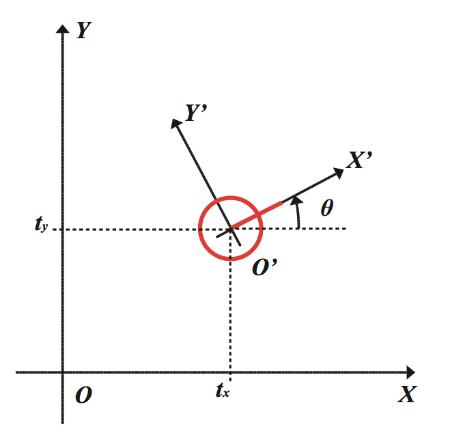
\includegraphics[height=5cm]{figures/2DCoordinate.png}
	\caption{2D坐标系转换}
\end{figure}
\begin{equation}
\left\{\begin{array}{l}{x_{w}=x_{r} \cos \theta-y_{r} \sin \theta+t_{x}} \\ {y_{w}=x_{r} \sin \theta-y_{r} \cos \theta+t_{y}}\end{array}\right.
\end{equation}
我们可以将其写成矩阵形式:
\begin{equation}
\vec{x_{w}}=\vec{R x_{r}}+\vec{t}\label{2dtranslate matrix}
\end{equation}
其中,
\begin{equation}
\mathbf{R}=\left[ \begin{array}{cc}{\cos \theta} & {-\sin \theta} \\ {\sin \theta} & {\cos \theta}\end{array}\right]
\end{equation}
\begin{equation}
\mathbf{t}=\left[t_{x}, t_{y}\right]^{T}
\end{equation}
$\vec R$是一个正交阵,我们称其为旋转矩阵,$\vec t$是平移向量。通过旋转矩阵$\vec{R}$和向量$\vec{t}$,我们准确的描述出局部坐标系的性质。
\subsection{变换矩阵和齐次坐标}
确实,公式\ref{2dtranslate matrix}表达了2D空间的旋转和平移,不过这里还存在一个问题:变换并不是一个线性的变换。假如我们进行了如下两次变换:$\vec R_1,\vec t_1$和$\vec R_2,\vec t_2$,满足:
\begin{equation}
\vec b = \vec R_1 \vec a + \vec t_1,\quad \vec c=\vec R_2 \vec b + \vec t_2
\end{equation}
从$\vec a$到$\vec c$的变换:
\begin{equation}
\vec c=\vec R_2(\vec R_1 \vec a + \vec t_1) + \vec t_2
\end{equation}
可以看到,这样的形式在多次坐标变换之后会变得十分复杂,但我们通过引入齐次坐标,并将变换矩阵重写一下就会发现:
\begin{equation}
\left[ \begin{array}{l}{b} \\ {1}\end{array}\right]=\left[ \begin{array}{ll}{R_{2\times 2}} & {t_{2\times 1}} \\ {0^{T}} & {1}\end{array}\right] \left[ \begin{array}{l}{a} \\ {1}\end{array}\right] = T_{3\times 3} \left[ \begin{array}{l}{a} \\ {1}\end{array}\right]
\end{equation}
我们将a的齐次坐标形式写作 $\vec{\widetilde{a}}$,可得:
\begin{equation}
\vec{\widetilde{c}} =\vec{ T_{cb}T_{ba}}\vec{\widetilde{a}}
\end{equation}
看,齐次坐标能够化简计算难度,通过将一个二维向量末尾添加1,将其变成三维向量,然后将旋转和平移写进同一个矩阵里面,让整个变成一个线性关系。我们称T为\textbf{变换矩阵(Transform Matrix)}。\par
\subsection{三维空间位姿表示}
上面介绍了二维空间的位姿描述,以此类推的话,三维空间的位姿表示也很简单:
\begin{equation}
\boldsymbol{T}=\left[ \begin{array}{ll}{\boldsymbol{R}_{3 \times 3}} & {\boldsymbol{t}_{3 \times 1}} \\ {\mathbf{0}_{1 \times 3}^{T}} & {I_{1 \times 1}}\end{array}\right]
\end{equation}
我们现在有了旋转矩阵来描述旋转,有了变换矩阵来描述一个6自由度的刚体运动,但是请注意,旋转矩阵有9个参数,而旋转只有三个自由度,这样的表达是冗余的;同时变换矩阵有16个参数,而刚体运动只有6个自由度,这样的描述也是冗余的。下面介绍其他几种更紧凑的旋转表示方法。
\subsubsection{欧拉角}
旋转矩阵虽然能够描述旋转,但是非常不直观,人们很难通过这个旋转矩阵想象出这个旋转怎么变换的。而欧拉角提供了一种非常直观的方式来描述旋转,把三维旋转分解成绕不同轴的旋转:偏航角、俯仰角、滚转角。\par
\begin{itemize}
\item 偏航角:绕物体的Z轴旋转
\item 偏航角:绕旋转之后的Y轴旋转
\item 滚转角:绕旋转之后的X轴旋转
\end{itemize}
\begin{figure}[htb]
	\centering
	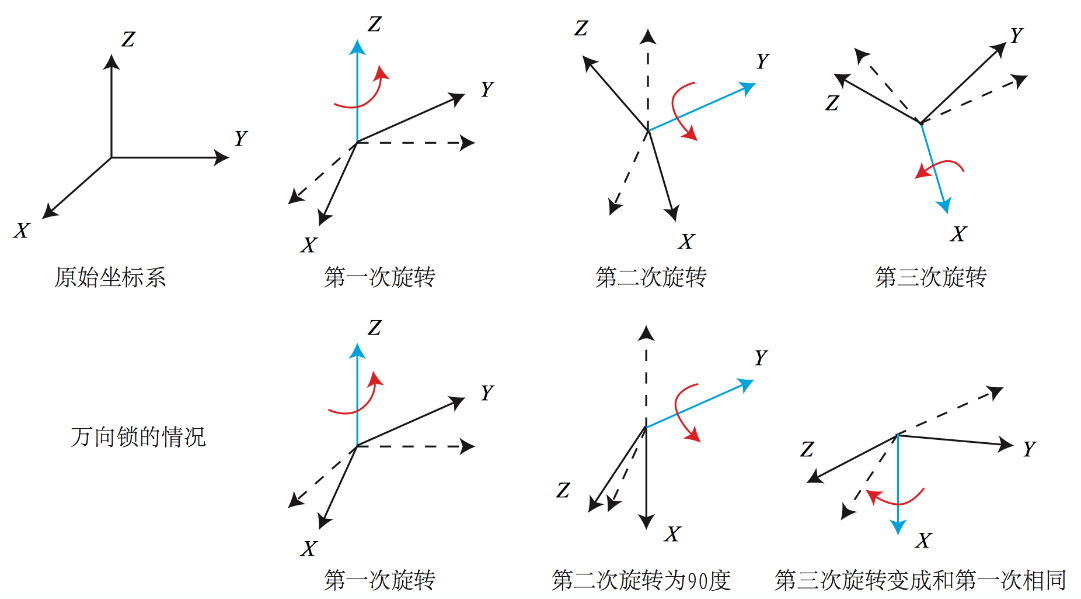
\includegraphics[height=5cm]{figures/GimbalLock.png}
	\caption{万向锁示意图}
\end{figure}\par
因此我们可以用这样一个三维的向量描述任意的旋转,我们能非常直观的想象出旋转的过程。但欧拉角有一个缺陷——万向锁问题(Gimbal Lock):在俯仰角为时,第一次旋转与第三次旋转将变成同一个,这就使得由三维旋转变成了两次旋转,丢失了一个自由度。这被称为奇异性问题,在其他形式的欧拉角中也同样存在。理论上可以证明,只要是通过三个实数来描述三维旋转,就会存在奇异性问题,因此,我们在后面的研究将不会采用欧拉角来表达姿态。
\subsubsection{四元数}
旋转矩阵用9个量描述3个自由度的旋转,具有冗余性;欧拉角和旋转向量是紧凑的,但是具有奇异性。事实上,我们找不到不带奇异性的三维向量表达方式\cite{rotationgroup}。四元数相较于欧拉角不存在万向锁问题,是一种紧凑易于迭代的姿态表示方法,相较于旋转向量,四元数最直观的好处就是省空间,因为一个旋转向量用9个分量来描述,但旋转只有三个自由度,而三个量来描述旋转会遇到奇异性问题,因此我们考虑使用四个量来刻画旋转。
四元数是一种扩展的复数,一个四元数拥有一个实部和三个虚部:
\begin{equation}
q=q_{0}+q_{1} i+q_{2} j+q_{3} k
\end{equation}
其中,i, j, k为四元数的三个虚部,这三个虚部满足以下关系式:
\begin{equation}
\left\{\begin{array}{c}{i^{2}=j^{2}=k^{2}=-1} \\ {i j=k, j i=-k} \\ {j k=i, j k=-i} \\ {k i=j, i k=-j}\end{array}\right.
\end{equation}
我们能用单位四元数表示三维空间中的任意一个旋转,单位四元数是模长为1的四元数。假设某个旋转是绕单位向量$\boldsymbol{n}=\left[n_{x}, n_{y}, n_{z}\right]^{T}
$为轴旋转$\theta$,那么这个旋转用四元数可表示为:
\begin{equation}
\mathbf{q}=\left[\cos \frac{\theta}{2}, n_{x} \sin \frac{\theta}{2}, n_{y} \sin \frac{\theta}{2}, n_{z} \sin \frac{\theta}{2}\right]^{T}
\end{equation}
反之,通过任意单位四元数,可以计算对应的转轴与夹角:
\begin{equation}
\left\{\begin{array}{c}{\theta=2 \cos ^{-1} q_{0}} \\ {\left[n_{x}, n_{y}, n_{z}\right]^{T}=\frac{\left[q_{1}, q_{2}, q_{3}\right]^{T}}{\sin \frac{\theta}{2}}}\end{array}\right.
\end{equation}
\subsubsection{旋转向量}
我们知道,任何一个旋转都可以用一个\textbf{转轴}和一个\textbf{旋转角}来刻画。可以设想这么一个向量,它的方向和旋转轴的方向一致,它的长度和旋转角度的大小一致,我们称这样的向量为\textbf{旋转向量(Axis-Angle)}。这种方法只需要三个量就能表示旋转,再加上表示位置的平移向量,正好6个参数表达一个6自由度的位姿变换。\par
那么剩下的问题是,旋转向量和旋转矩阵是如何转换的呢?旋转向量并不能直接用来计算,它只是旋转的一种表示方法,具体的计算过程还要转化为旋转矩阵。从旋转向量到旋转矩阵的过程由\textbf{罗德里格斯公式(Rodrigues's Formula)}给出:
\begin{equation}
\boldsymbol{R}=\cos \theta \boldsymbol{I}+(1-\cos \theta) \boldsymbol{n} \boldsymbol{n}^{T}+\sin \theta \boldsymbol{n}^{\wedge}\label{rodrigues}
\end{equation}
符号$\wedge$是向量到反对称矩阵转换符,例如:
\begin{equation}
	[a_1,a_2,a_3]^\wedge = \begin{bmatrix}
	0 & -a_3 & a_2\\
	a_3& 0& -a_1\\
	-a_2& a_1& 0
	\end{bmatrix}\label{fanduichen}
\end{equation}

\section{李群和李代数}
\subsection{李群和李代数的引入}
在前面我们介绍了旋转矩阵和变换矩阵的定义,但是旋转矩阵和变换矩阵都是对加法不封闭的。也就是说两个旋转矩阵相加,就不再是一个旋转矩阵了。这就给优化的过程造成了困难,因为求导这个过程无从定义。在SLAM系统中,位姿是未知的,我们需要解决一个相机到底处于什么样的位姿才能和当前观测最符合的问题,因此我们在初步得到旋转的表示之后,我们还要对它进行优化。在进行优化的时候,旋转矩阵本身是有一定约束:要求正交且行列式为1,再加上之前的对加法不封闭的性质会使得优化变得十分困难。所以我们这个时候就要通过李群李代数之间的转换关系,把位姿估计变成无约束优化问题进行求解。
\subsection{李群的定义}
群是\textbf{一种集合}再加上\textbf{一种运算}的代数结构,如果把某个集合记作A,运算记作$\cdot$这样群可以记作G=(A,$\cdot$)。一个群要求运算满足下面几个条件:
\begin{enumerate}
\item 封闭性:$\forall a_{1}, a_{2} \in A, \quad a_{1}\cdot a_{2} \in A$
\item 结合律:$\forall a_{1}, a_{2}, a_{3} \in A,\quad \left(a_{1} \cdot a_{2}\right) \cdot a_{3}=a_{1} \cdot\left(a_{2} \cdot a_{3}\right)$
\item 幺元:  $\exists a_{0} \in A,$ $\forall a \in A,\quad a_{0} \cdot a=a \cdot a_{0}=a$
\item 逆:   $\forall a \in A, \exists a^{-1} \in A,$\quad $a \cdot a^{-1}=a_{0}$
\end{enumerate}
常见的群比如正数的加法(幺元为0)($\mathbb{Z}$,+),去掉0之后的有理数乘法(幺元为1)$(\mathbb{Q} \verb|\|0,\times)$。\par
事实上,旋转矩阵也构成了群,也就是所谓的\textbf{特殊正交群SO(3)},而变换矩阵构成了\textbf{特殊欧式群SE(3)}:
\begin{equation}
SO(3)=\left\{\mathbf{R} \in \mathbb{R}^{3 \times 3} | \mathbf{RR}^{T}=\mathbf{I}, \operatorname{det}(\mathbf{R})=1\right\}
\end{equation}
\begin{equation}
SE(3)=\left\{\mathbf{T}=\left[ \begin{array}{ll}{\boldsymbol{R}} & {\boldsymbol{t}} \\ {\mathbf{0}^{T}} & {1}\end{array}\right] \in \mathbb{R}^{4 \times 4} | \boldsymbol{R} \in SO(3), \boldsymbol{t} \in \mathbb{R}^{3}\right\}
\end{equation}
可以知道,这两个群对乘法都是成群的,但是对加法却是不封闭的。换句话说,对于任意两个旋转矩阵$\boldsymbol{R_1}$,$\boldsymbol{R_2}$,相加之后将不再表示一个旋转矩阵:
\begin{equation}
\boldsymbol{R_1}+\boldsymbol{R_2}\notin \boldsymbol{SO(3)}
\end{equation}\par
\textbf{李群}就是一种具有连续性质的群。比如整数群$\mathbb{z}$那样离散的群没有连续性质,不能称作李群。而SO(3)和SE(3)我们可以想象到一个刚体连续的运动旋转,因此它们都是李群。回到我们最初的问题,旋转矩阵和变换矩阵对加法不封闭,而且自身带有约束,造成了我们后期优化困难,因此我们希望能将对SO(3)和SE(3)的优化,转化成一种无约束的优化问题。这就是引入李代数的目的。
\subsection{李代数的引入}
考虑任意的旋转矩阵\textbf{R},我们知道它满足:
\begin{equation}
	\boldsymbol{RR^T}=\boldsymbol{I}
\end{equation}
我们把R当做某个相机的旋转,它会随着时间变化而变化,也就是\textbf{R}是时间的函数。由于\textbf{R}(t)仍然是旋转矩阵,故:
\begin{equation}
	\boldsymbol{R}(t)\boldsymbol{R}(t)^T=\boldsymbol{I}
\end{equation}
现在在等式两边对时间求导,得:
\begin{equation}
	\dot{\boldsymbol{R}}(t)\boldsymbol{R}(t)^T+\boldsymbol{R}(t)\dot{\boldsymbol{R}}(t)^T=0
\end{equation}
整理得:
\begin{equation}
\dot{\boldsymbol{R}}(t)\boldsymbol{R}(t)^T=-\left(\dot{\boldsymbol{R}}(t)\boldsymbol{R}(t)^T\right)^T
\end{equation}
可以看到$\dot{\boldsymbol{R}}(t)\boldsymbol{R}(t)^T$是一个反对称矩阵。回忆一下公式\ref{fanduichen},我们可以定义一个符号$\vee$来表示从矩阵到向量的转换:
\begin{equation}
	\vec{a}^\wedge = \vec{A}=\begin{bmatrix}
	0 & -a_3 & a_2\\
	a_3& 0& -a_1\\
	-a_2& a_1& 0
	\end{bmatrix}, \vec{A}^\vee = \vec{a}
\end{equation}
由于$\dot{\boldsymbol{R}}(t)\boldsymbol{R}(t)^T$是一个反对称矩阵,因此我们可以找到一个三维向量,$\phi(t)\in \mathbb{R}^3$与该矩阵对应:
\begin{equation}
	\dot{\boldsymbol{R}}(t)\boldsymbol{R}(t)^T = \phi(t)^\wedge
\end{equation}
等式两边右乘一个$\vec{R}(t)$,有:
\begin{equation}
	\dot{\boldsymbol{R}}(t)=\phi(t)^\wedge \vec{R}(t)=\left[ \begin{array}{ccc}{0} & {-\phi_{3}} & {\phi_{2}} \\ {\phi_{3}} & {0} & {-\phi_{1}} \\ {-\phi_{2}} & {\phi_{1}} & {0}\end{array}\right] \boldsymbol{R}(t)\label{Rqiudao}
\end{equation}
我们惊喜的发现,本来旋转矩阵对时间的导数是难以计算的,通过引入一个三维向量我们成功的将旋转矩阵的求导转化为了旋转矩阵左乘一个$\phi(t)^\wedge$即可。\par
我们假设在0时刻的时候旋转矩阵为$\vec{R}(0)=\vec{I}$,$\vec{R}(t)$在0时刻的泰勒展开为:
\begin{equation}
\begin{aligned} \boldsymbol{R}(t) & \approx \boldsymbol{R}\left(t_{0}\right)+\dot{\boldsymbol{R}}\left(t_{0}\right)\left(t-t_{0}\right) \\ &=\boldsymbol{I}+\boldsymbol{\phi}\left(t_{0}\right)^{\wedge}(t) \end{aligned}
\end{equation}
同样的,在时间$t_0$附近,$\phi(t_0)=\phi_0$,那么根据公式\ref{Rqiudao}:
\begin{equation}
\dot{\boldsymbol{R}}(t)=\boldsymbol{\phi}\left(t_{0}\right)^{\wedge} \boldsymbol{R}(t)=\boldsymbol{\phi}_{0}^{\wedge} \boldsymbol{R}(t)
\end{equation}
这是一个微分方程,已知初值为$\vec{R}(0)=I$,则:
\begin{equation}
\boldsymbol{R}(t)=\exp \left(\phi_{0}^{\wedge} t\right)
\end{equation}
也就是:
\begin{equation}
\boldsymbol{R}=\exp \left(\phi^{\wedge}\right)\label{expyingshe}
\end{equation}
公式\ref{expyingshe}中的exp并不是常规的指数函数,而是矩阵的指数函数。它实际上反应的是一种映射,称之为\textbf{指数映射}。
\subsection{李代数的定义}
李代数由一个向量空间$\mathbb{V}$,一个数域$\mathbb{F}$和一个二元运算[,]组成,记作$\mathfrak{g}$。李代数满足以下性质:
\begin{enumerate}
\item 封闭性 $\forall X, Y \in \mathbb{V},[X, Y] \in \mathbb{V}$
\item 双线性 $\forall X, Y, Z \in \mathbb{V}, a, b \in \mathbb{F},$有:\\
$[a \mathrm{X}+\mathrm{bY}, \mathrm{cZ}+\mathrm{d} \mathrm{W}]=a c[\mathrm{X}, \mathrm{Z}]+b c[Y, Z]+a d[X, W]+b d[Y, W]$
\item 自反性 $\forall X \in \mathbb{V},[X, X]=0$
\item 雅克比等价 $\forall X, Y, Z \in \mathbb{V},[X,[Y,Z]]+[Z,[Y X]]+[Y,[Z,X]]=\vec{0}$
\end{enumerate}
其中二元运算符$[,]$被称作李括号。例如三维向量$\mathbb{R}^3$上的叉积$\times$是一种李括号,因此$(\mathbb{R}^3,\mathbb{R},\times)$构成了一个李代数。
\subsection{李代数$\mathfrak{so}$(3)}
我们之前提到的$\phi$,事实上就是一种李代数。那么这个李代数对应的李括号是什么呢?首先令:
\begin{equation}
	\Phi=\phi^{\wedge}=\left[ \begin{array}{ccc}{0} & {-\phi_{3}} & {\phi_{2}} \\ {\phi_{3}} & {0} & {-\phi_{1}} \\ {-\phi_{2}} & {\phi_{1}} & {0}\end{array}\right] \in \mathbb{R}^{3 \times 3}
\end{equation}
那么两个向量$\phi_{1},\phi_{2}$的李括号为:
\begin{equation}
\left[\phi_{1}, \phi_{2}\right]=\left(\Phi_{1} \Phi_{2}-\Phi_{2} \Phi_{1}\right)^\vee
\end{equation}

\subsection{李代数$\mathfrak{se}$(3)}
对于SE(3),它也有对应的李代数$\mathfrak{se}$(3),记作$\xi$,$\xi \in \mathbb{R}^6$。同时,也有对应的$\wedge$符号:
\begin{equation}
\mathfrak{se}(3)=\left\{
	\xi=\left[ \begin{array}{l}{\rho} \\ {\phi}\end{array}\right] \in \mathbb{R}^{6},\rho \in \mathbb{R}^{3},\phi \in \mathfrak{so}(3),\xi^{\wedge}=\left[ \begin{array}{ll}{\phi^{\wedge}} & {\rho} \\ {0^{T}} & {0}\end{array}\right] \in \mathbb{R}^{4\times4}
	\right\}
\end{equation}
与$\boldsymbol{R}=\exp \left(\phi^{\wedge}\right)$对应的,若变换矩阵为T,SE(3)下也有相应的指数映射关系:
\begin{equation}
	\vec{T}=\exp(\xi^\wedge)
\end{equation}
可以看到$\xi$是一个六维向量,其中前三维是平移(并不是真正的平移,还需要做一些变换),记作$\rho$,后三维是旋转,记作$\phi$,也就是旋转向量对应的李代数。同时我们扩展了$\wedge$的含义,表示"从向量到矩阵"的含义,$\vee$表示"从矩阵到向量"。李代数$\mathfrak{se}(3)$也有对应的李括号:
\begin{equation}
\left[\xi_{1}, \xi_{2}\right]=\left(\xi_{1}^\wedge \xi_{2}^\wedge-\xi_{2}^\wedge \xi_{1}^\wedge\right)^{\vee}
\end{equation}
\section{指数映射和对数映射}
说了这么多,其实对于$\exp(\phi^\wedge)$以及$\exp(\xi^\wedge)$是怎么个映射关系依然没有交代清楚。下面我们就来推导一下$SO(3)$下的指数映射关系。
\subsection{SO(3)的指数映射}
我们知道任意矩阵的指数映射可以写成一个泰勒展开,其结果仍是一个矩阵:
\begin{equation}
	\exp(\vec{A})=\sum_{n=0}^{\infty}\frac{1}{n!}\vec{A}^n
\end{equation}
同样的对于$exp(\phi^\wedge)$,我们也有如下定义:
\begin{equation}
\exp(\vec{\phi^\wedge})=\sum_{n=0}^{\infty}\frac{1}{n!}(\phi^\wedge)^n
\end{equation}
我们知道$\phi$是一个三维向量,我们可以定义它的模长为$\theta$,方向为$\vec{a}$,对于$\vec{a}$,我们知道它有如下两条性质:
\begin{equation}
\left\{\begin{aligned}
	\vec{a}^\wedge\vec{a}^\wedge=&\vec{a}\vec{a}^T-\vec{I}\\
\vec{a}^\wedge\vec{a}^\wedge\vec{a}^\wedge=&-\vec{a}^\wedge
\end{aligned}\right.
\end{equation}
于是:
\begin{equation*}
\begin{aligned} 
\exp \left(\phi^{\wedge}\right) &=\exp \left(\theta a^{\wedge}\right)=\sum_{n=0}^{\infty} \frac{1}{n !}\left(\theta a^{\wedge}\right)^{n} \\
&=I+\theta a^{\wedge}+\frac{1}{2 !} \theta^{2} a^{\wedge} a^{\wedge}+\frac{1}{3 !} \theta^{3} a^{\wedge} a^{\wedge} a^{\wedge}+\frac{1}{4 !} \theta^{4}\left(a^{\wedge}\right)^{4}+\ldots\\
&=a a^{T}-a^{\wedge} a^{\wedge}+\theta a^{\wedge}+\frac{1}{2 !} \theta^{2} a^{\wedge} a^{\wedge}-\frac{1}{3 !} \theta^{3} a^{\wedge}-\frac{1}{4 !} \theta^{4}\left(a^{\wedge}\right)^{2}+\ldots \\ 
&=a a^{T}+\left(\theta-\frac{1}{3 !} \theta^{3}+\frac{1}{5 !} \theta^{5}-\dots\right) a^{\wedge}-\left(1-\frac{1}{2 !} \theta^{2}+\frac{1}{4 !} \theta^{4}-\ldots\right) a^{\wedge} a^{\wedge}\\
&=a^{\wedge} a^{\wedge}+I+\sin \theta a^{\wedge}-\cos \theta a^{\wedge} a^{\wedge}\\
&=(1-\cos \theta) a^{\wedge} a^{\wedge}+I+\sin \theta a^{\wedge} \\
&=\cos \theta I+(1-\cos \theta) a a^{T}+\sin \theta a^{\wedge}
\end{aligned}
\end{equation*}

最后我们可以推导出:
\begin{equation}
\exp \left(\theta \boldsymbol{a}^{\wedge}\right)=\cos \theta \boldsymbol{I}+(1-\cos \theta) \boldsymbol{a} \boldsymbol{a}^{T}+\sin \theta \boldsymbol{a}^{\wedge}
\end{equation}
对照公式\ref{rodrigues}:
\begin{equation*}
	\boldsymbol{R}=\cos \theta \boldsymbol{I}+(1-\cos \theta) \boldsymbol{n} \boldsymbol{n}^{T}+\sin \theta \boldsymbol{n}^{\wedge}
\end{equation*}
我们发现SO(3)对应的李代数原来是旋转向量!$\phi$的模就是旋转的角度,方向就是旋转轴。到现在为止,我们搞清楚了$\phi \rightarrow \vec{R}$,那么$\vec{R}\rightarrow \phi$又是如何计算的呢?可以通过:
\begin{equation}
	\phi = \ln{R}^\vee=\left(
	\sum_{n=0}^{\infty}\frac{(-1)^n}{n+1}(\vec{R}-\vec{I})^{n+1}
	\right)^\vee
\end{equation}
来计算。这里直接给出结果:
\begin{equation}
	\theta=\arccos{\frac{tr(\vec{R})-1}{2}}
\end{equation}
关于转轴$\vec n$,由于转轴上的向量在旋转后不变,因此:
\begin{equation}
	\vec{Rn}=\vec{n}
\end{equation}
求解$\vec n$然后归一化即可。
\subsection{SE(3)的指数映射}
对于六维向量$\xi$,符号$\wedge$表示:
\begin{equation}
\xi=\left[ \begin{array}{l}{\rho} \\ {\phi}\end{array}\right], \quad \xi^{\wedge}=\left[ \begin{array}{cc}{\phi^{\wedge}} & {\rho} \\ {0^{T}} & {0}\end{array}\right]
\end{equation}
这里直接给出SE(3)上的指数映射:
\begin{equation}
\begin{aligned}
\exp \left(\xi^{\wedge}\right)&=\left[ \begin{array}{cc}{\sum_{n=0}^{\infty} \frac{1}{n !}\left(\phi^{\wedge}\right)^{n}} & {\sum_{n=0}^{\infty} \frac{1}{(n+1) !}\left(\phi^{\wedge}\right)^{n} \rho} \\ {0^{\mathrm{T}}} & {1}\end{array}\right]\\
&\triangleq \left[ \begin{array}{cc}{\boldsymbol{R}} & {\boldsymbol{J} \rho} \\ {\mathbf{0}^{\mathrm{T}}} & {1}\end{array}\right]=\boldsymbol{T}
\end{aligned}
\end{equation}
可以看到,$\vec{T}$的左上角由$\xi$的后三维,也就是$\mathfrak{so}$(3)的指数映射计算得到。右上角由$\xi$的前三维左乘一个$\vec J$矩阵得到:
\begin{equation}
\vec J=\frac{\sin \theta}{\theta} I+\left(1-\frac{\sin \theta}{\theta}\right) a a^{T}+\frac{1-\cos \theta}{\theta} a^{\wedge}
\label{matrixJ}
\end{equation}\par
至于对数映射,也就是从矩阵到向量的映射,不必再经过泰勒展开,直接根据变换矩阵$\vec T$的形式计算即可。具体来说,就是由$\vec T$的左上角$\vec R$来计算$\xi$的后三维$\phi$,至于$\rho$,可以由方程:
\begin{equation}
	\vec{t=J\rho}
\end{equation}
来计算。其中$\vec J$已经由\ref{matrixJ}给出。\par
至此,SO(3)和SE(3)上的李群李代数和相互的转化关系:指数映射,对数映射都已经介绍完毕,如图
\begin{figure}
	\centering
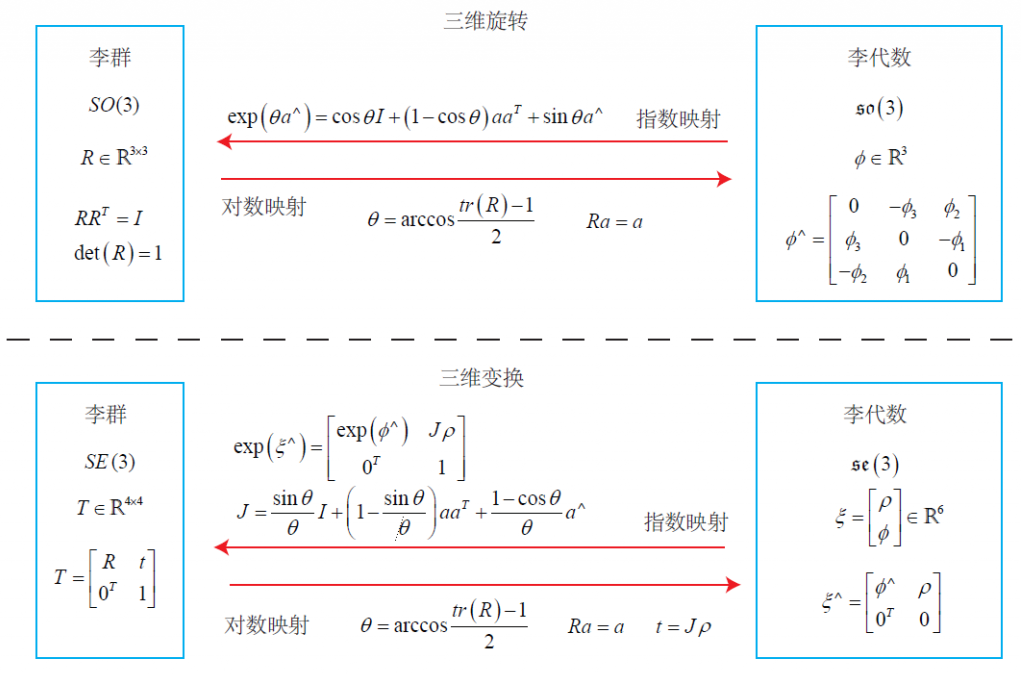
\includegraphics[height=9cm]{figures/lie.png}
\caption{SO(3),SE(3),$\mathfrak{so(3),se(3)}$的对应关系}
\end{figure}
\section{扰动模型}
接下来我们简单介绍一下SE(3)和SO(3)如何利用扰动模型求导。
\subsection{SO(3)上的扰动模型}
假设我们对一个空间点$\vec p$进行了旋转,得到了$\vec Rp$,那么要计算旋转之后的点的坐标相对于旋转的导数该如何计算呢?我们可以考虑对$\vec R$进行一个微小的扰动,也可以说是增量$\delta R$,假设这个扰动对应的李代数是$\varphi$,然后对$\varphi$求导,得:
\begin{equation}
\frac{\partial(\boldsymbol{R} \boldsymbol{p})}{\partial \boldsymbol{\varphi}}=\lim _{\varphi \rightarrow 0} \frac{\exp \left(\boldsymbol{\varphi}^{\wedge}\right) \exp \left(\boldsymbol{\phi}^{\wedge}\right) \boldsymbol{p}-\exp \left(\boldsymbol{\phi}^{\wedge}\right) \boldsymbol{p}}{\varphi}
\end{equation}
对小量进行泰勒展开,得:
\begin{equation}
\begin{aligned}
\frac{\partial(\boldsymbol{R p})}{\partial \varphi} &=\lim _{\varphi \rightarrow 0} \frac{\exp \left(\varphi^{\wedge}\right) \exp \left(\phi^{\wedge}\right) \boldsymbol{p}-\exp \left(\phi^{\wedge}\right) \boldsymbol{p}}{\varphi} \\ & \approx \lim _{\varphi \rightarrow 0} \frac{\left(1+\varphi^{\wedge}\right) \exp \left(\phi^{\wedge}\right) \boldsymbol{p}-\exp \left(\phi^{\wedge}\right) \boldsymbol{p}}{\varphi} \\ &=\lim _{\varphi \rightarrow 0} \frac{\varphi^{\wedge} \boldsymbol{R p}}{\varphi}=\lim _{\varphi \rightarrow 0} \frac{-(\boldsymbol{R p})^{\wedge} \varphi}{\varphi}=-(\boldsymbol{R p})^{\wedge}
\end{aligned}
\end{equation}
这里可能比较难以理解的是第三行,$\phi^\wedge\vec R \vec p$实际上等于$\phi\times (\vec R \vec p)$,根据叉乘的交换律,也就是$-(\vec R \vec p)\times \phi$,即:$-(\vec R \vec p)^\wedge \phi$。这个求导的结果是一个3$\times$3的矩阵,表示旋转后的三个维度,分别关于小扰动的三个分量的导数。
\subsection{SE(3)上的扰动模型}
同样的,假设我们对空间点$\vec p$进行了一次旋转+平移,得到了$\vec T p$\footnote{此处$\vec p$是齐次坐标。},现在,给T左乘一个扰动$\Delta T$=$\exp{(\delta \xi^\wedge)}$,设扰动的李代数$\delta \xi=[\delta \rho,\delta \phi]^T$,因此关于扰动的导数为:
\begin{equation}
\begin{aligned}
\frac{\partial(T p)}{\partial \delta \xi}
&=\lim _{\delta \xi \rightarrow 0} \frac{\exp \left(\delta \xi^{\wedge}\right) \exp \left(\xi^{\wedge}\right) p-\exp \left(\xi^{\wedge}\right) p}{\delta \xi} \\
& \approx \lim _{\delta \xi \rightarrow 0} \frac{\left(I+\delta \xi^{\wedge}\right) \exp \left(\xi^{\wedge}\right) p-\exp \left(\xi^{\wedge}\right) p}{\delta \xi} \\
&=\lim _{\delta \xi \rightarrow 0} \frac{\delta \xi^{\wedge} \exp \left(\xi^{\wedge}\right) p}{\delta \xi}\\
&=\lim _{\delta \xi \rightarrow 0} \frac{\left[ \begin{array}{cc}{\delta \phi^{\wedge}} & {\delta \rho} \\ {\mathbf{0}^{T}} & {0}\end{array}\right] \left[ \begin{array}{c}{\boldsymbol{R} p+t} \\ {\mathbf{1}}\end{array}\right]}{\delta \boldsymbol{\xi}}\\
&=\lim _{\delta \xi \rightarrow 0} \frac{\left[ \begin{array}{c}{\delta \phi^{\wedge}(R p+t)+\delta \rho} \\ {0}\end{array}\right]}{\delta \xi}=\left[ \begin{array}{cc}{I} & {-(R p+t)^{\wedge}} \\ {0^{T}} & {0^{T}}\end{array}\right] \triangleq(T p)^{\circ}
\end{aligned}
\label{equ:raodong}
\end{equation}
$\circ$代表了将一个齐次坐标空间点变换成一个4$\times$6的矩阵。
























% !TeX root = ../main.tex
\chapter{相机和图像}
\section{相机模型}
视觉SLAM本质上是对空间点,相机位姿的求解。SLAM系统的输入是时序的图片,因此我们有必要了解一下现实中的三维信息是如何被转化成图片上一个个像素点的。我们通过对相机的建模,来模仿现实相机的行为,从而帮助我们理解相机的工作原理。现在我们就来介绍一种最常用的相机模型:\textbf{针孔相机模型(Pinhole camera)}
\subsection{针孔相机模型}
针孔相机模型模型描述的是一束光线通过针孔之后,在针孔背后投影成像。由于获得好的成像效果,我们在相机的前方加了透镜。透镜的加入对成像过程中光线的传播会产生新的影响:一是透镜自身的形状对光线传播的影响,二是在机械组装过程中,透镜和成像平面不可能完全平行,这也会使得光线穿过透镜投影到成像平面时的位置发生变化。这个现象叫做畸变,因此在使用相机前,对测量精度较高的相机,还要做非线性标定,即测出畸变参数。因此我们的建模分成两部分:对针孔模型的建模和对相机畸变的建模。
\begin{figure}
	\centering
	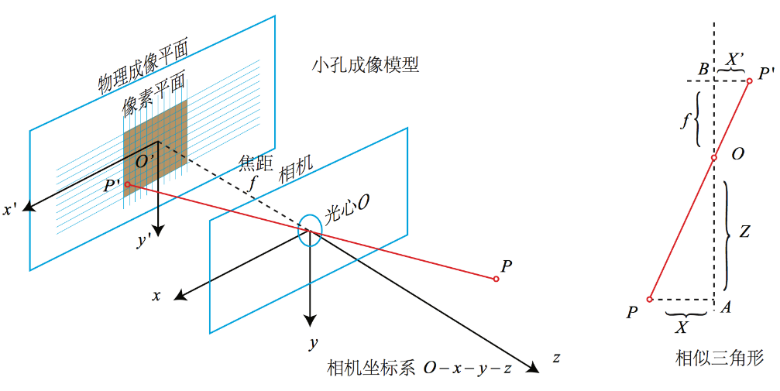
\includegraphics[height=5cm]{figures/pinholemodule.png}
	\caption{针孔模型}
\end{figure}
下面我们对这个针孔模型进行几何建模。设O–xyz为相机坐标系,现实世界中的空间点P,经过小孔O投影之后,落在成像平面O'-x'y'z'上,为P'。设P,P'的坐标分别为$[X,Y,Z]^{T},\left[X^{\prime}, Y^{\prime}, Z^{\prime}\right]^{T}$,成像焦距为f。那么根据三角形相似,则有:
\begin{equation*}
\frac{Z}{f}=-\frac{X}{X^{\prime}}=-\frac{Y}{Y^{\prime}}
\end{equation*}
这里的负号表示成的是倒立的像。为了简化计算,我们常常会把这个负号去掉,把成像平面对称至相机前方:
\begin{equation}
\frac{Z}{f}=\frac{X}{X^{\prime}}=\frac{Y}{Y^{\prime}}\label{Ptochengxiang}
\end{equation}
式\ref{Ptochengxiang}描述了空间点P经过小孔成的像之间的空间几何关系。但是在相机坐标系中,我们需要的是像素点的坐标,所以我们需要进一步变换。\par
设成像平面上的像素平面O–uv,则像素平面上点P'的像素坐标为:$[u, v]^{T}$。像素坐标系定义方式:原点位于图像成像平面左上角,$u$轴x轴平行且与向右,$v$轴与y平行且向下。在像素坐标系和成像平面之间通常相差了一个\textbf{缩放}和一个\textbf{原点的平移},我们设像素坐标在轴上缩放了$\alpha$倍,在轴上缩放了$\beta$倍,同时原点平移了$\left[c_{x}, c_{y}\right]$。这样我们就得到了像素坐标系和成像平面的关系,那么P'的成像坐标和其像素坐标关系如下:
\begin{equation}
\left\{\begin{array}{l}{u=\alpha X^{\prime}+c_{x}} \\ {v=\beta Y^{\prime}+c_{y}}\end{array}\right.
\label{chengxiangtopixel}
\end{equation}
将\ref{Ptochengxiang}代入上式子,并且将$\alpha f$合成为$f_x$,将$\beta f$合成为$f_y$得:
\begin{equation}
\left\{\begin{array}{l}{u=f_{x} \frac{X}{Z}+c_{x}} \\ {v=f_{y} \frac{Y}{Z}+c_{y}}\end{array}\right.
\end{equation}
写成矩阵的形式就是:
\begin{equation}
\left( \begin{array}{l}{u} \\ {v} \\ {1}\end{array}\right)=\frac{1}{Z} \left( \begin{array}{ccc}{f_{x}} & {0} & {c_{x}} \\ {0} & {f_{y}} & {c_{y}} \\ {0} & {0} & {1}\end{array}\right) \left( \begin{array}{l}{X} \\ {Y} \\ {Z}\end{array}\right) \triangleq \frac{1}{Z}\boldsymbol{KP}
\label{cameratopix}
\end{equation}
我们称上式中的\textbf{K}为相机的内参矩阵。一般来说,相机的内参在出厂之后是固定的,不会在使用过程中发生变化。有的厂商会告诉你相机的内参,而有时需要你自己确定相机的内参,也就是所谓的标定。可以看到,若三维空间内有一点$P=[x,y,z]$,先计算其在归一化平面上的坐标,也就是$[\frac{x}{z},\frac{y}{z},1]$,然后再乘以相机内参矩阵\textbf{K}就能得到像素位置。\par
现在我们来更深入的讨论一下这个流程。考虑一个世界坐标系下的点$P_w$,相机坐标系在世界坐标系下的位姿是$T$。公式\ref{cameratopix}中的$P$是相机坐标系下的坐标。因此若要计算$P_w$的像素坐标,需要先进行变换:
\begin{equation}
\left( \begin{array}{c}{u} \\ {v} \\ {1}\end{array}\right)=
\underbrace{
\left( \begin{array}{ccc}{f_{\alpha}} & {0} & {u_{0}} \\ {0} & {f_{\beta}} & {v_{0}} \\ {0} & {0} & {1}\end{array}\right)
\underbrace{\frac{1}{z_{c}}\overbrace{\left[ \begin{array}{cc}{\boldsymbol{R}} & {\boldsymbol{t}} \\ {\boldsymbol{0}^{T}} & {1}\end{array}\right]
\overbrace{\left( \begin{array}{c}{x_{w}} \\ {y_{w}} \\ {z_{w}} \\ {1}\end{array}\right)}^\text{世界坐标系}}^\text{相机坐标系}}_\text{归一化平面坐标}}_\text{像素平面坐标}\label{totalequation}
\end{equation}
上式从相机坐标系变成归一化坐标系的过程中省略了第四维,方便起见,以后齐次坐标和非齐次坐标的转换不再指出。事实上,将式\ref{totalequation}中$\frac{1}{z_c}$去掉也无妨,因为对于齐次坐标同乘以一个非零的数,结果并不变,无非是最后像素坐标再同除最后一维即可。因此,上式可简单写成:
\begin{equation}
	\boldsymbol{P_{uv}=KTP_w}
\end{equation}
至此,针孔相机的成像我们便介绍清楚了。
\section{畸变}
前面我们说道,为了获得好的成像效果,我们在相机的前方安装透镜,这就会产生了畸变。
其中,由于透镜形状引起的畸变称为径向畸变。在针孔模型中,一条直线投影到像素平面还是一条直线,可是在实际拍摄的照片中,直线往往会变成曲线,越靠近图像的边缘,这种现象越明显。由于实际加工制作的透镜往往是中心对称的,这使得不规则的畸变通常中心对称。它们主要分为两大类:桶形畸变和枕形畸变,如图\ref{jingxiangjibian}所示:
\begin{figure}
	\centering
	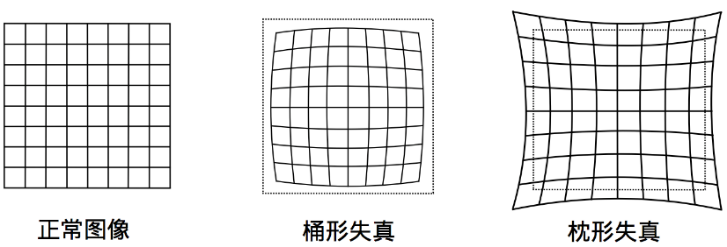
\includegraphics[height=4cm]{figures/jibian.png}
	\caption{径向畸变}\label{jingxiangjibian}
\end{figure}\par
除了透镜形状引起的畸变外,由于相机透镜安装的位置与成像平面不平行引起的畸变称之为切向畸变:
\begin{figure}
	\centering
	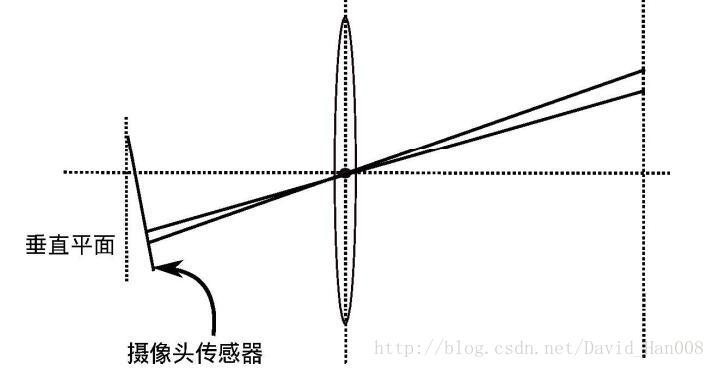
\includegraphics[height=4cm]{figures/qiexiangjibian.jpg}
	\caption{切向畸变}\label{qiexiangjibian}
\end{figure}\par
在SLAM特征点匹配过程中,这些错位的点是不可用的,我们要想办法去除掉畸变。我们知道平面上的任意一点p可以表示为$[x,y]^T$,也可以把它写成极坐标的形式$[r,\theta]^T$ ,其中$r$表示点$p$离坐标系原点的距离,$\theta$表示和水平轴的夹角。径向畸变可看成坐标点沿着长度方向发生了变化$\delta r$,也就是其距离原点的长度发生了变化。切向畸变可以看成坐标点沿着切线方向发生了变化,也就是水平夹角发生了变化$\delta \theta$。对于径向畸变,无论是桶形畸变还是枕形畸变,由于它们都是随着离中心的距离增加而增加。可以用一个多项式函数来描述畸变前后的坐标变化:这类畸变可以用和距中心距离有关的二次及高次多项式函数进行纠正:
\begin{equation}
\begin{aligned} x_{\text {corrected}} &=x\left(1+k_{1} r^{2}+k_{2} r^{4}+k_{3} r^{6}\right) \\ y_{\text {corrected}} &=y\left(1+k_{1} r^{2}+k_{2} r^{4}+k_{3} r^{6}\right) \end{aligned}
\end{equation}
其中$[x,y]^T$ 是未纠正的点的坐标,$[x_{corrected},y_{corrected}]^T$ 是纠正后的点的坐标,注意它们都是归一化平面上的点,而不是像素平面上的点。\par
对于畸变较小的图像中心区域,畸变纠正主要是k1起作用。而对于畸变较大的边缘区域主要是k2 起作用。普通摄像头用这两个系数就能很好的纠正径向畸变。对畸变很大的摄像头,比如鱼眼镜头,可以加入k3 畸变项对畸变进行纠正。\par
另一方面,对于切向畸变,可以使用另外的两个参数$p1 ,p2$来进行纠正:
\begin{equation}
\begin{aligned} c_{\text {corrected}} &=x+2 p_{1} x y+p_{2}\left(r^{2}+2 x^{2}\right) \\ y_{\text {corrected}} &=y+p_{1}\left(r^{2}+2 y^{2}\right)+2 p_{2} x y \end{aligned}
\end{equation}\par
对于相机坐标系中的一点$P(X,Y,Z)$,我们能够通过以下几个步骤找到这个点在像素平面上的正确位置:\par
\begin{enumerate}
\item 将三维空间点投影到归一化图像平面。设它的归一化坐标为$[x,y]^T$。
\item 对归一化平面上的点进行径向畸变和切向畸变纠正。
\begin{equation}
\begin{aligned} x_{\text {corrected}} &=x\left(1+k_{1} r^{2}+k_{2} r^{4}+k_{3} r^{6}\right)+2 p_{1} x y+p_{2}\left(r^{2}+2 x^{2}\right) \\ y_{\text {corrected}} &=y\left(1+k_{1} r^{2}+k_{2} r^{4}+k_{3} r^{6}\right)+p_{1}\left(r^{2}+2 y^{2}\right)+2 p_{2} x y \end{aligned}
\end{equation}
\item 将纠正后的点通过内参数矩阵投影到像素平面,得到该点在图像上的正确位置。
\begin{equation}
\begin{aligned} u &=f_{x} x_{\text {corrected}}+c_{x} \\ v &=f_{y} y_{\text {corrected}}+c_{y} \end{aligned}
\end{equation}
\item 在上面的纠正畸变的过程中,使用了五个畸变项。实际应用中,可以灵活选择纠正模型,对于畸变不大的情况,只选择k1 ,p1 , p2 这三项即可。
\end{enumerate}
我们从头来总结一下单目相机的成像过程:
\begin{enumerate}
\item 首先,世界坐标系下有一个固定的点$P$,世界坐标为$P_w$;
\item 相机坐标系的运动由$\vec{R},\vec{t}$或变换矩阵$\vec{T} \in SE(3)$描述。$P_w$的相机坐标为:$P_{c}=R P_{w}+t$;
\item 将$P_c$把它们投影到归一化平面$Z=1$上,得到$\tilde{P_c}=[X / Z, Y / Z, 1]^{T}$
\item 最后,$P_c$的归一化坐标经过内参变换后,得到它的像素坐标:$\vec{P_{uv}=K\tilde{P_c}}$ 。
\end{enumerate}\par
\subsection{相机的标定}
目前主流的相机标定方式是采用张友正标定法\cite{zhang1999flexible}。畸变参数一般在SLAM系统中是已知的,如果不知道的话,MATLAB和Opencv中都有封装好的相机标定的工具包,简单几步操作就能快速标定相机。
% !TeX root = ../main.tex
\chapter{特征点的提取与匹配}
\section{图像特征介绍}
图像匹配技术是计算机视觉领域的技术重要组成之一。图像匹配这项技术主要应用于目标识别、图像拼接、自动跟踪定位等研究。而基于特征点的图像匹配则是一种十分有效的方法。进行特征匹配的话,一般分为三个步骤,特征提取、特征描述和特征匹配。具体就是通过检测关键点,然后提取描述向量,最后来建立局部特征描述子,再进行特征匹配的过程。
\section{特征检测子}
\subsection{Harris 角点检测}
角点往往是两条边缘的交点,它是两条边缘方向变换的一种表示,因此其两个方向的梯度变换通常都比较大并且容易检测到。这里我们理解一下角点检测的算法。\par
\subsubsection{角点检测基本原理:}\par
人们通常通过在一个小的窗口区域内观察点的灰度值大小来识别角点,如果往任何方向移动窗口都会引起比较大的灰度变换那么往往这就是我们要找的角点。如下图:\par
\begin{figure}[htbp]
\centering
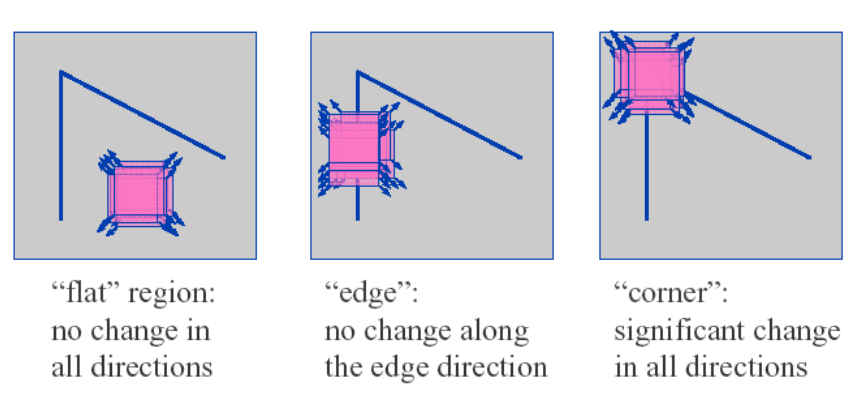
\includegraphics[height=5cm]{figures/Harris1.png}
\caption{角点的选择}
\end{figure}
\subsubsection{角点检测基本流程}
使用角点检测算子,对图像的每个像素计算角点响应函数(Corner Response Function ),阈值化角点响应函数,根据实际情况选择阈值,对阈值化的角点响应函数进行非极大值抑制,并获取非零点作为角点。
\subsubsection{Harris角点\cite{harris1988combined}}
下面我们看一下Harris的数学公式:
\begin{equation}
E(u,v)=\sum_{x}\sum_{y} w(x,y)[I(x+u,y+v)-I(x,y)]^{2}\label{Harris}
\end{equation}\par
式中$E(u,v)$即为角点响应函数,事实上被叫做窗口响应函数可能更合适,因为实际上$E(u,v)$计算的是一个5\times5或者7\times7的窗口。$x,y$为要计算的像素点。$I(x,y)$为该点的灰度值。$w(x,y)$为窗函数,可以理解为每个像素点的加权系数。
\begin{figure}[htbp]
	\centering
	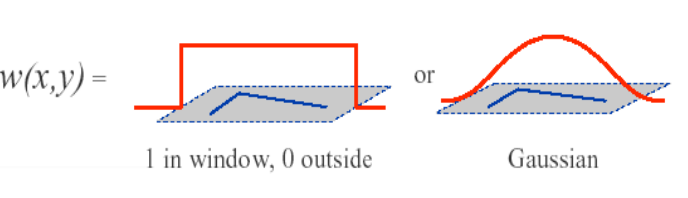
\includegraphics[height=3cm]{figures/Harris2.png}
	\caption{窗口函数}
\end{figure}
可以想象的到,对于平滑的,灰度值相对稳定的区域,该响应函数趋近于0;对于边缘区域,该响应函数在垂直于边缘方向上响应大,平行于边缘区域响应小;对于角点区域,无论什么方向响应都很大。道理是这个道理,但是给定上面的式子,变化u,v时,我们不能很直观的看出$E(u,v)$的变化。所以,我们要对上式进行一些变化和近似。使用泰勒级数展开,并忽略非线性项:
\begin{equation}
\begin{aligned}
I(x+u, y+v) &\approx I(x, y)+u I_{x}+v I_{y}+\omicron\left(I_x^{2},I_y^{2}\right)\\
&=I(x, y)+u I_{x}+v I_{y}
\end{aligned}
\end{equation}\par
由于图像的检测算子都很小,对上式做泰勒一阶展开是合理的,故响应函数可化为:
\begin{equation}
\begin{aligned}
E(u,v)=&\sum_{x,y} w(x,y) [I(x+u, y+v)-I(x, y)]^{2} \\
\approx&\sum_{x,y}w(x,y)\left[I(x, y)+u I_{x}+v I_{y}-I(x, y)\right]^{2}\\
=&\sum_{x,y}w(x,y) \left(u^{2} I_{x}^{2}+2 u v I_{x} I_{y}+v^{2} I_{y}^{2} \right)\\
=&\sum_{x,y}w(x,y) \left[ \begin{array}{cc}{u} & {v}\end{array}\right] \left[ \begin{array}{cc}{I_{x}^{2}} & {I_{x} I_{y}} \\ 
{I_{x} I_{y}} & {I_{y}^{2}}\end{array}\right] \left[ \begin{array}{c}{u} \\ 
{v}\end{array}\right]\\
=&\left[ \begin{array}{cc}{u} & {v}\end{array}\right]M\left[\begin{array}{c}{u}\\{v}\end{array}\right]
\end{aligned}
\end{equation}
其中:
\begin{equation}
M=\sum_{x, y} w(x, y) \left( \begin{array}{cc}{I_{x}^{2}} & {I_{x} I_{y}} \\ {I_{x} I_{y}} & {I_{y}^{2}}\end{array}\right)=\left( \begin{array}{cc}{\sum_{W} I_{x}^{2}} & {\sum_{W} I_{x} I_{y}} \\ {\sum_{W} I_{x} I_{y}} & {\sum_{W} I_{y}^{2}}\end{array}\right)=\left[ \begin{array}{cc}{A} & {C} \\ {C} & {B}\end{array}\right]
\end{equation}
故:
\begin{equation}
	E(u,v) \approx Au^{2}+2Cuv+Bv^{2}
\end{equation}
由公式\ref{Harris}可以看到,这样的函数在三维空间上起码是非负定的,如图\ref{ercixing}所示:
\begin{figure}[htbp]
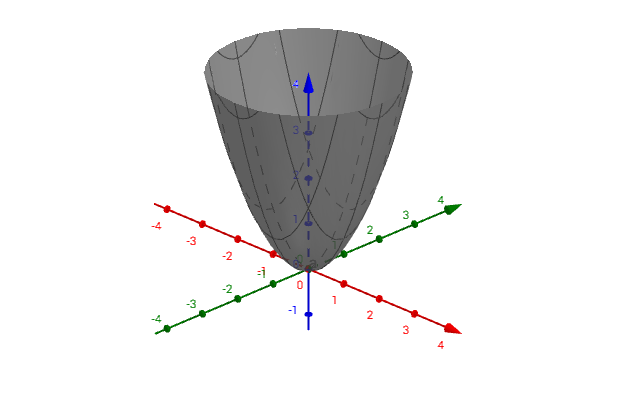
\includegraphics[height=5cm]{figures/ercixing.png}
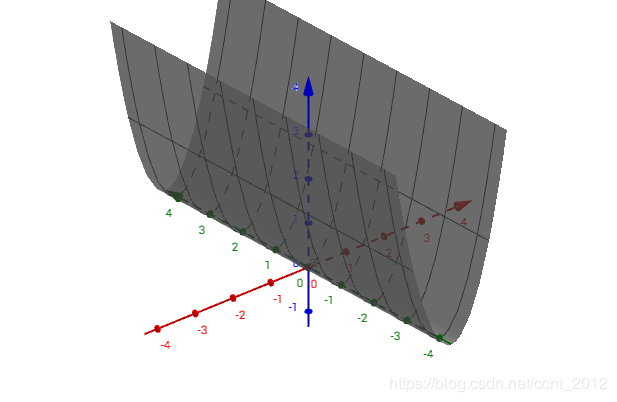
\includegraphics[height=5cm]{figures/ercixing1.png}
\caption{$E(u,v)$图像}
\label{ercixing}
\end{figure}\\
因此问题就变成了究竟怎样形式的E(u,v)的图像,才能算作一个特征点。直观上讲,一个角点应该无论在哪个方向上,响应函数$E$都应有一个大的变化。我们的也可以这么说:为了使响应函数$E$在角点邻域内有较大的变化量,M应该有两个较大的特征值。论文\cite{harris1988combined}指出,二次型矩阵的两个特征值$\lambda_1$和$\lambda_2$与点邻域的性质有如下关系:
\begin{itemize}
	\item 若$\lambda_1 \approx 0$,$\lambda_2\approx 0$,则表示图像在此处变化不大;
	
	\item 若$\lambda_1 \approx 0$且$\lambda_2$具有很大的正值,则表示检测到了边缘;
	
	\item 若$\lambda_1$,$\lambda_2$都很大,则表示检测到了角点;
\end{itemize}
但是实际在应用中,由于计算特征值比较慢,我们转而计算函数$R$来得到结果。其中$\kappa$是灵敏度系数,$\kappa$越小越敏感,一般来说$\kappa=0.04$。
\begin{equation}
	R = \lambda_1\lambda_2-\kappa(\lambda_1+\lambda_2)^2=det(M)-\kappa trace^2(M)
\end{equation}
因此,算法并不直接计算特征值,而是通过矩阵的行列式和迹来测量角点,从而大大提高了计算效率。\par
算法在计算完图像中的角点之后,图像上某些区域可能会出现角点十分密集的情况,这时候就要进行\textbf{非最大值抑制(Non-maximal Suppression)}。也就是说只保留局部区域中响应最大的特征点,从而避免匹配的时候重复检测。\par
\begin{figure}[htbp]
	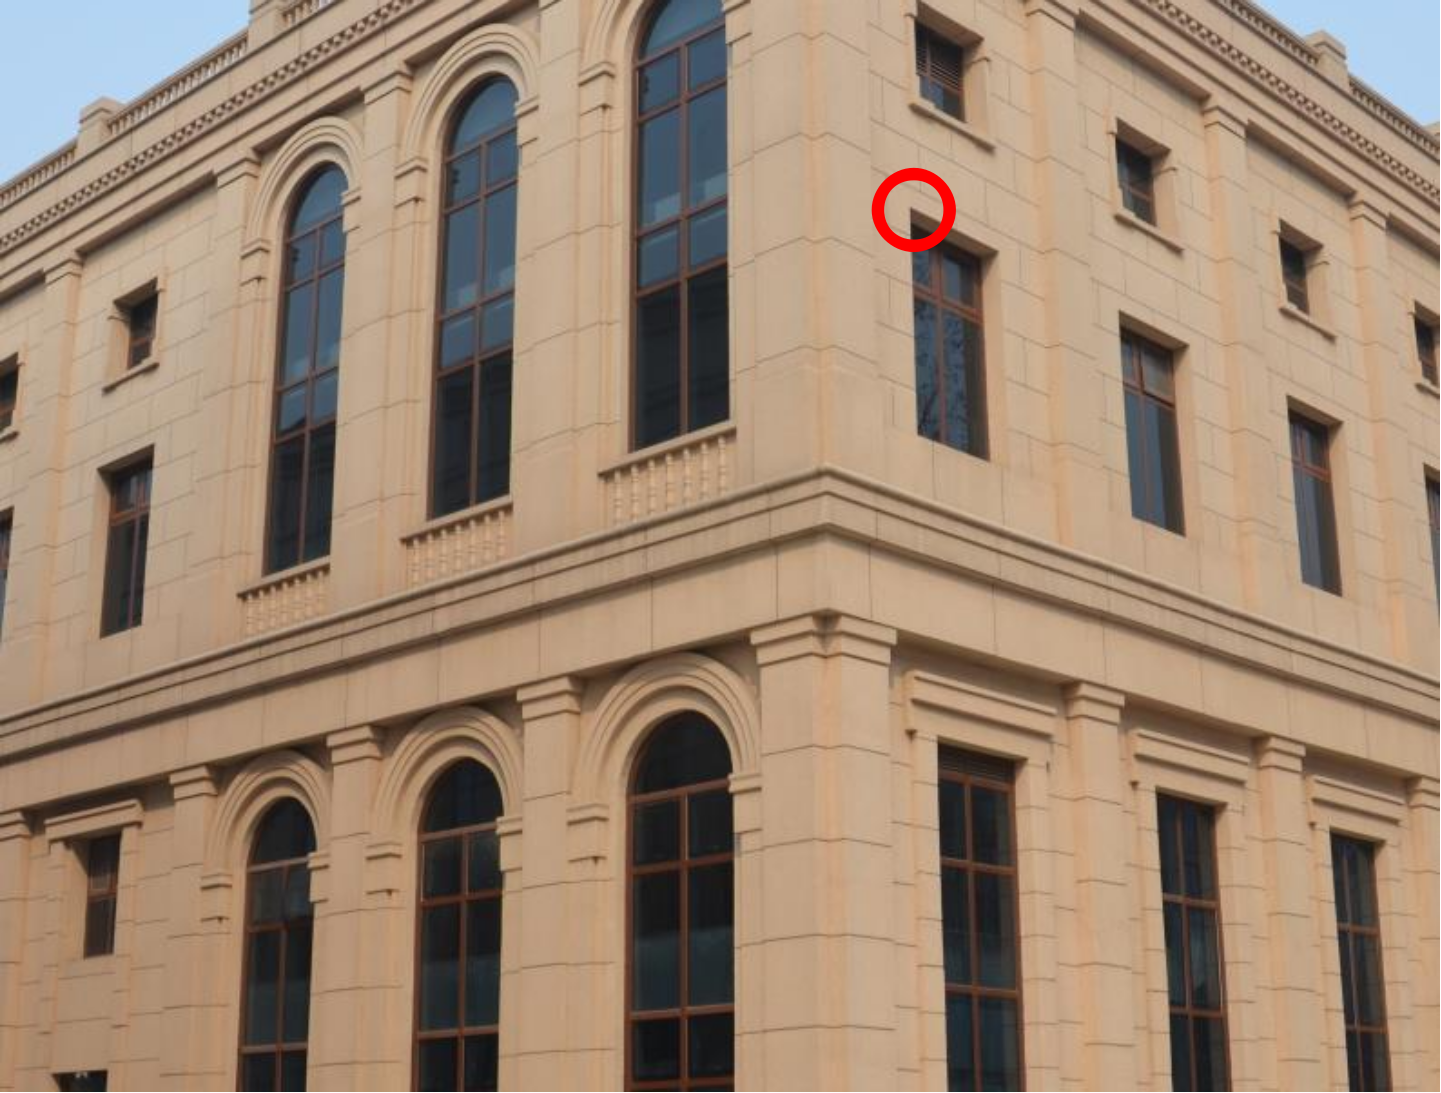
\includegraphics[height=5cm]{figures/LoG1.png}
	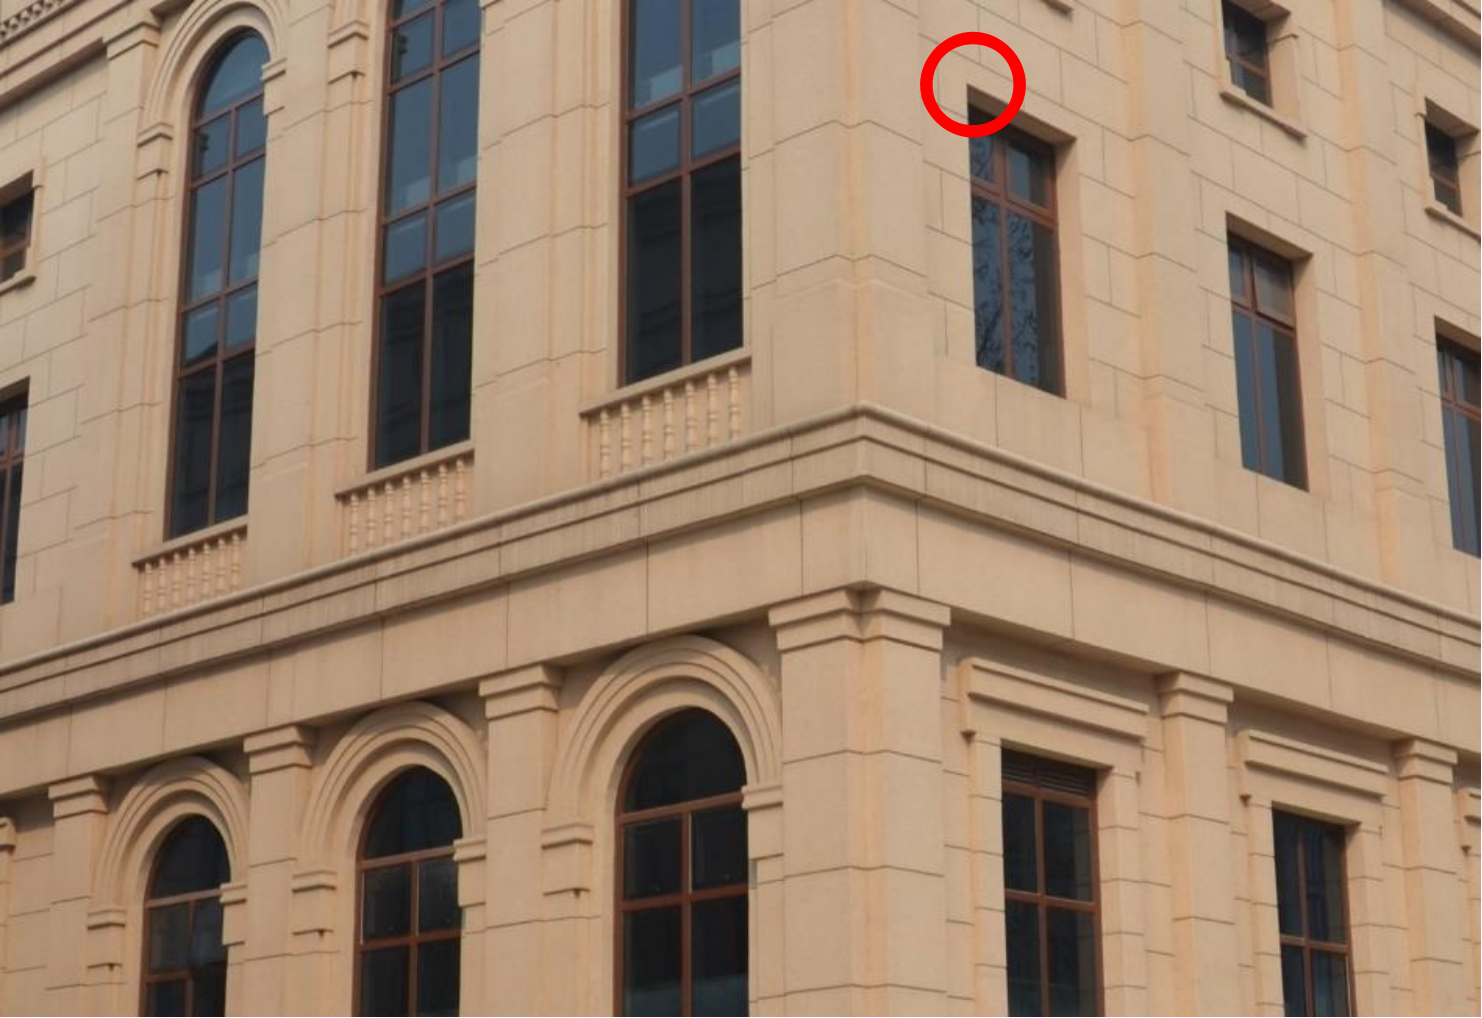
\includegraphics[height=5cm]{figures/LoG2.png}
	\caption{Harris角点不具有尺度不变性}
	\label{HarrisScale}
\end{figure}
这样,基于Harris角点的特征点检测方法已经介绍完了,但是这种角点并不完美。最大的问题就是Harris角点的检测窗口大小是固定的,也就是说Harris角点不具有尺度不变性。如图\ref{HarrisScale}可以看出来。左侧图像期望一个小的检测窗口,而右侧图像期待一个大的检测窗口。显然,在尺度变化较大的图像中,Harris角点并不能胜任检测工作,由此我们引出基于LoG的多尺度特征检测子。\par

\subsection{基于LoG的多尺度特征检测子}
\subsubsection{Laplace算子}
Laplace算子简单来说是两个梯度算子的点乘:
\begin{equation*}
\triangle=\nabla \cdot \nabla=\nabla^{2}=\left[\frac{\partial}{\partial x_{1}}, \cdots, \frac{\partial}{\partial x_{N}}\right] \left[ \begin{array}{c}{\frac{\partial}{\partial x_{1}}} \\ {\vdots} \\ {\frac{\partial}{\partial x_{N}}}\end{array}\right]=\sum_{n=1}^{N} \frac{\partial^{2}}{\partial x_{n}^{2}}
\end{equation*}
对于图像处理来说,一般用到的是二维的Laplace算子:
\begin{equation*}
\triangle=\nabla \cdot \nabla=\nabla^{2}=\left[\frac{\partial}{\partial x} \frac{\partial}{\partial y}\right] \left[ \begin{array}{c}{\frac{\partial}{\partial x}} \\ {\frac{\partial}{\partial y}}\end{array}\right]=\frac{\partial^{2}}{\partial x^{2}}+\frac{\partial^{2}}{\partial y^{2}}
\end{equation*}
对于函数$f(x,y)$应用Laplace算子:
\begin{equation*}
\triangle f(x, y)=\frac{\partial^{2} f}{\partial x^{2}}+\frac{\partial^{2} f}{\partial y^{2}}
\end{equation*}
对于离散的情况,二阶微分就变成了二阶差分。\par
我们先来看看在一维情况下将一阶差分:
\begin{equation*}
\nabla f[n]=f[n+1]-f[n]
\end{equation*}
那么一维的二阶差分就是:
\begin{equation*}
	\begin{aligned}
	\triangle f[n]=&\nabla(\nabla f[n])=\nabla f[n]-\nabla f[n-1]\\
	=&(f[n+1]-f[n])-(f[n]-f[n-1])\\
	=&f[n+1]-2 f[n]+f[n-1]
	\end{aligned}
\end{equation*}
因此,在一维情况下,Laplace算子可以理解成一维的卷积,其卷积核是$[1,-2,1]$。\par
在二维情况下,Laplace算子是两个维度中两个二阶差分的总和:
\begin{equation}
\begin{aligned}
\triangle f[m, n]=&\triangle_{m}[f[m, n]]+\triangle_{n}[f[m, n]]\\
=&f[m+1, n]-2 f[m, n]+f[m-1, n]+f[m, n+1]-2 f[m, n]+f[m, n-1]\\
=&f[m+1, n]+f[m-1, n]+f[m, n+1]+f[m, n-1]-4 f[m, n]
\end{aligned}
\end{equation}
此操作也可以理解成二维的卷积,其卷积核是:
\begin{equation*}
\left[ \begin{array}{lll}{0} & {1} & {0} \\ {1} & {-4} & {1} \\ {0} & {1} & {0}\end{array}\right]
\end{equation*}
\subsubsection{LoG算子}
图像中的噪声和边缘一样会使图像产生灰度跳变,我们在使用Laplace算子检测边缘细节的同时,往往也增强了噪声,因此,如何区分开噪声和边缘是个问题。\par
为了在取得较好的检测同时把噪声干扰降到最低,可以先对有噪声的原始图像进行平滑滤波,然后再进行锐化处理增强边缘和细节。基于这一思想,Marr和Hildreth\cite{marr1980theory}提出了把高斯平滑算子和拉普拉斯锐化算子结合起来的方法,称之为拉普拉斯-高斯(LoG)算子。\par
高斯平滑算子:
\begin{equation}
G_{\sigma}(x, y)=\frac{1}{\sqrt{2 \pi \sigma^{2}}} \exp \left(-\frac{x^{2}+y^{2}}{2 \sigma^{2}}\right)
\end{equation}\par
LoG算子:
\begin{equation}
\triangle\left[G_{\sigma}(x, y) * f(x, y)\right]=\left[\triangle G_{\sigma}(x, y)\right] * f(x, y)=L o G * f(x, y)
\\
\end{equation}
\begin{equation}
\begin{aligned}
L o G \triangleq& \triangle G_{\sigma}(x, y)=\frac{\partial^{2}}{\partial x^{2}} G_{\sigma}(x, y)+\frac{\partial^{2}}{\partial y^{2}} G_{\sigma}(x, y)\\
=&\frac{x^{2}+y^{2}-2 \sigma^{2}}{\sigma^{4}} \exp \left(-\frac{x^{2}+y^{2}}{2 \sigma^{2}}\right)
\end{aligned}
\end{equation}\par
画出LoG算子的空间形状:
\begin{figure}[H]
	\centering
	\begin{subfigure}[ht]{0.3\textwidth}
		\centering
		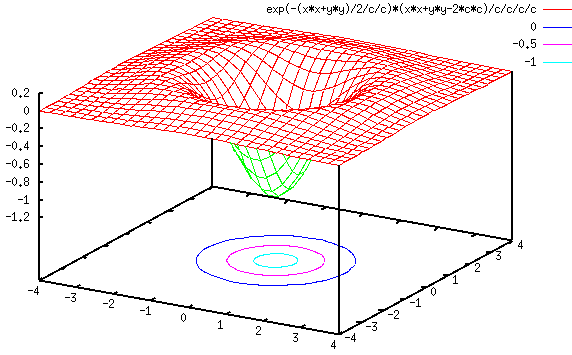
\includegraphics[height=0.7\textwidth]{figures/LoG_plot.png}
		\subcaption{连续空间表示}
	\end{subfigure}
\qquad \qquad \qquad
	\begin{subfigure}[ht]{0.3\textwidth}
		\centering
		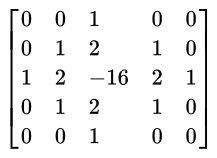
\includegraphics[height=0.7\textwidth]{figures/LoG_table}
		\subcaption{离散空间表示}
	\end{subfigure}
\caption{LoG算子空间表示}
\end{figure}
\begin{figure}[htbp]
\centering
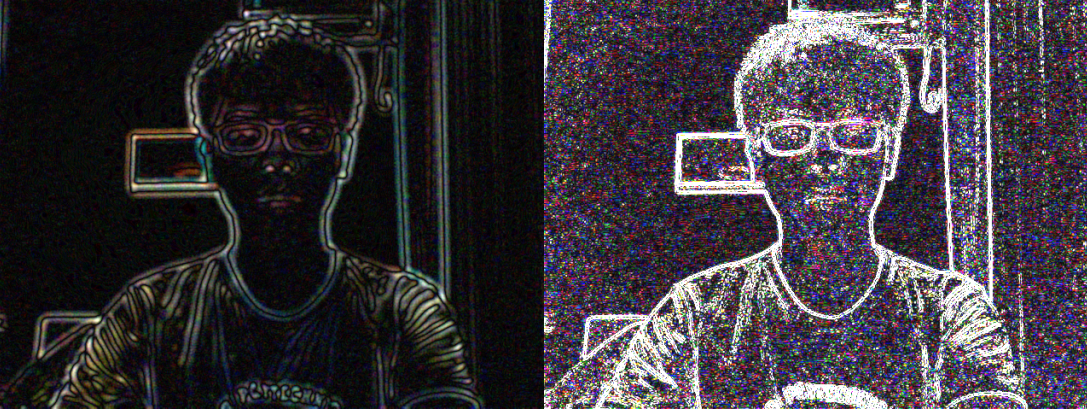
\includegraphics[height=3.5cm]{figures/LoG.png}
\caption{左:LoG算子\qquad \qquad \qquad \qquad 右:Laplace算子}
\end{figure}\par
可以看到,LoG算子显著减小了噪点对检测的影响。
\subsubsection{尺度空间}
为了解决一般角点不具有尺度不变性的问题,我们在此引入尺度空间:
\begin{equation}
L\left(x, y, \sigma_{D}\right)=I(x, y) * G\left(x, y, \sigma_{D}\right), \quad \sigma_{D} \in\left\{\sigma_{0}, \quad k \sigma_{0}, \quad k^{2} \sigma_{0}, \quad \dots\right\}
\end{equation}
尺度空间下的LoG算子:
\begin{equation}
\begin{aligned}
\nabla^{2} \mathrm{L}\left(x, y, \sigma_{\mathrm{D}}\right)=&\left(\frac{\partial^{2} \mathrm{L}\left(x, y, \sigma_{\mathrm{D}}\right)}{\partial x^{2}}+\frac{\partial^{2} \mathrm{L}\left(x, y, \sigma_{\mathrm{D}}\right)}{\partial y^{2}}\right)\\
=&\underbrace{\left(\frac{\partial^{2} \mathrm{G}\left(x, y, \sigma_{\mathrm{D}}\right)}{\partial x^{2}}+\frac{\partial^{2} \mathrm{G}\left(x, y, \sigma_{\mathrm{D}}\right)}{\partial y^{2}}\right)}_\text{多尺度LoG算子}*I(x,y)
\end{aligned}
\end{equation}
从公式可以看出,所谓尺度空间,就是用不同大小的高斯滤波核来对图像进行处理。如图\ref{differentkernalsize}所示:
\begin{figure}[H]
	\centering
	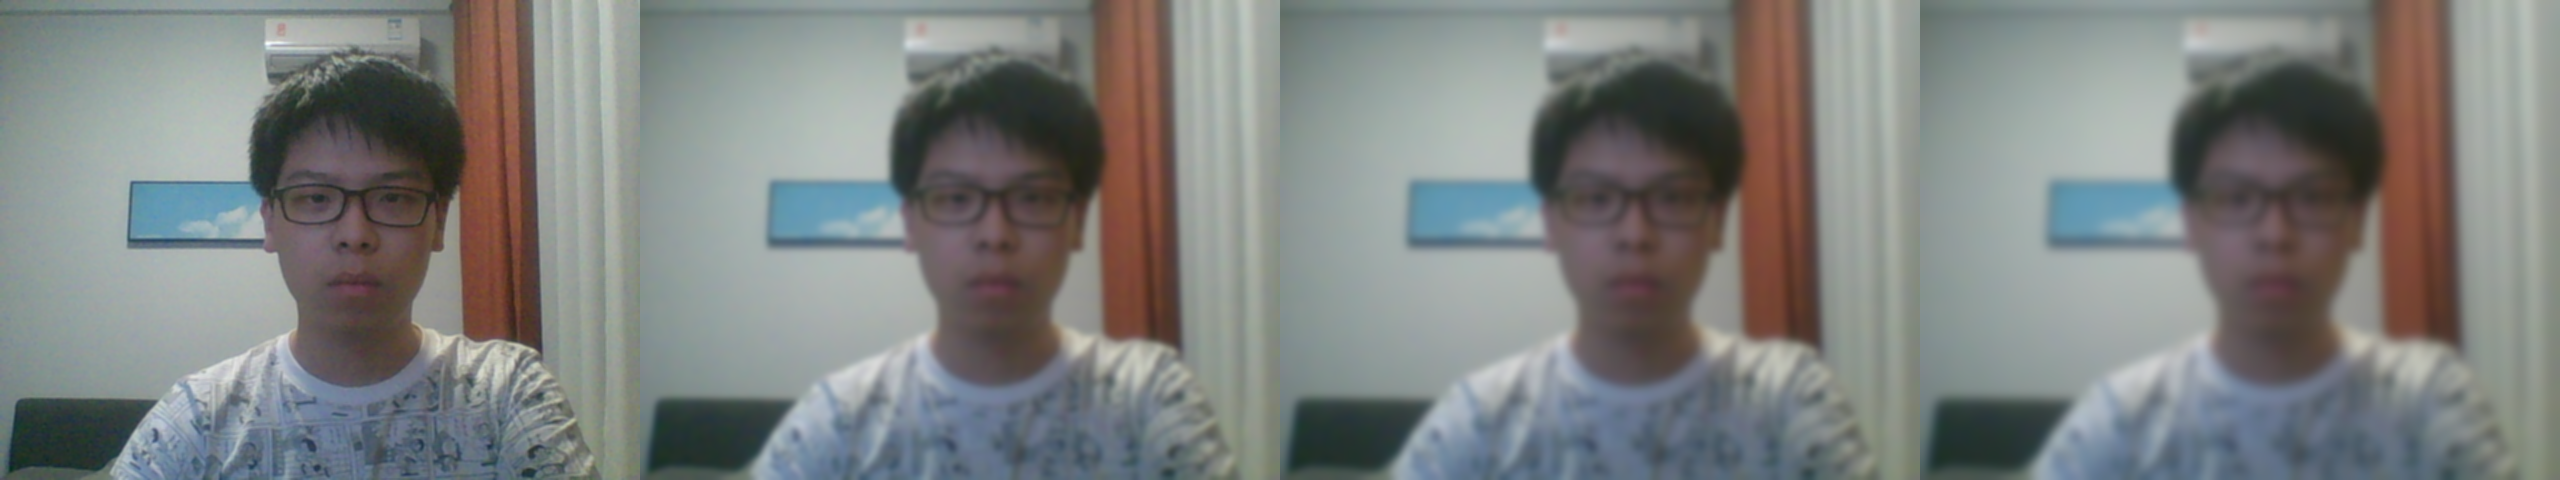
\includegraphics[height=3cm]{differentkernalsize.png}
	\caption{不同的高斯滤波核大小,从左至右依次是3$\times$3,11$\times$11,21$\times$21,25$\times$25}\label{differentkernalsize}
\end{figure}\par
可以看到滤波核越大,图像就越模糊。这实际上也是在模拟人类的视觉,因为距离越远,人看上去也越模糊。因此我们可以用不同滤波核来模拟不同的尺度。\par
但是这种多尺度的LoG算子有一个问题,不同尺度的LoG算子计算出来的响应值不具有可比性,因此我们需要对LoG算子进行归一化操作,才能够在不同尺度之间比较LoG算子的响应值,具体的做法就是将LoG算子乘上一个尺度:
\begin{equation}
\nabla_{\text { norm }}^{2} \mathrm{L}\left(x, y, \sigma_{\mathrm{D}}\right)= 
\underbrace{\sigma_{\mathrm{D}}^{2}\left(\frac{\partial^{2} \mathrm{G}\left(x, y, \sigma_{\mathrm{D}}\right)}{\partial x^{2}}+\frac{\partial^{2} \mathrm{G}\left(x, y, \sigma_{\mathrm{D}}\right)}{\partial y^{2}}\right)}_\text{尺度归一化LoG算子} * I(x, y)
\end{equation}
那么寻找特征点的过程,就可以转化为求解$| \nabla_{\text { nomm }}^{2} \mathbf{L}\left(x, y, \sigma_{\mathrm{D}}\right) |$最值的过程。\par
\subsection{基于DoG的多尺度特征检测子(sift)}
实际上这种基于LoG算子检测特征点的方法效果是很好的,但是它十分耗费计算资源。计算速度不快。于是Lowe\cite{lowe2004sift}提出相邻尺度的高斯差分(DoG)来近似LoG算法,也就是所谓的sift特征点。Difference of Gaussian(DoG)是高斯函数的差分。字面意思理解,首先将图像与两个方差不同的高斯函数进行卷积得到两幅滤波结果,然后再将图像相减,得到DoG的响应值图像。
\begin{equation}
\begin{aligned} g_{1}(x, y) &=G_{\sigma_{1}}(x, y) * f(x, y) \\ g_{2}(x, y) &=G_{\sigma_{2}}(x, y) * f(x, y) \end{aligned}
\end{equation}
则DoG表示为:
\begin{equation}
D o G \triangleq G_{\sigma_{1}}-G_{\sigma_{2}}=\frac{1}{\sqrt{2 \pi}}\left(\frac{1}{\sigma_{1}} e^{-\left(x^{2}+y^{2}\right) / 2 \sigma_{1}^{2}}-\frac{1}{\sigma_{2}} e^{-\left(x^{2}+y^{2}\right) / 2 \sigma_{2}^{2}}\right)
\end{equation}
\begin{figure}[H]
	\centering
	\begin{subfigure}[ht]{0.3\textwidth}
		\centering
		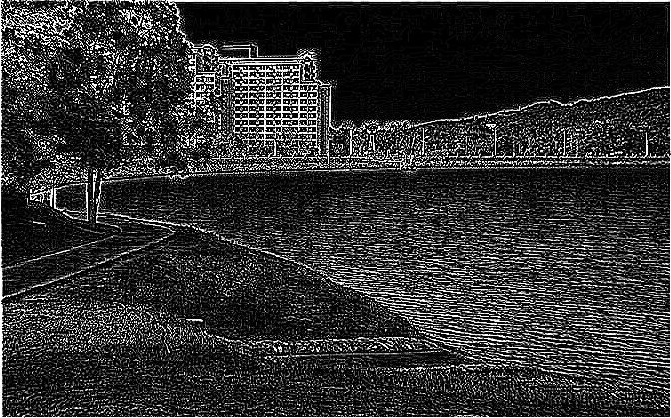
\includegraphics[height=0.7\textwidth]{figures/DoG1.png}
		\subcaption{$\sigma_1=$0.3,$\sigma_2=$0.4}
	\end{subfigure}
	\begin{subfigure}[ht]{0.3\textwidth}
		\centering
		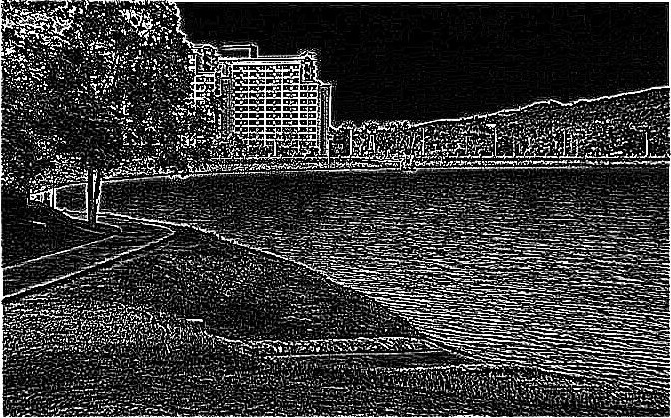
\includegraphics[height=0.7\textwidth]{figures/DoG2.png}
		\subcaption{$\sigma_1=$0.6,$\sigma_2=$0.7}
	\end{subfigure}
	\begin{subfigure}[ht]{0.3\textwidth}
	\centering
	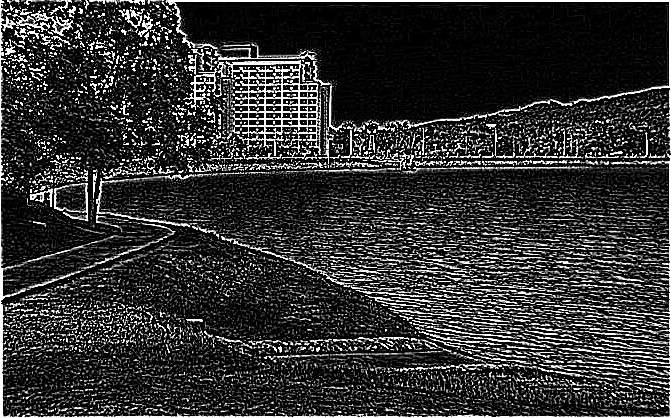
\includegraphics[height=0.7\textwidth]{figures/DoG3.png}
	\subcaption{$\sigma_1=$0.7,$\sigma_2=$0.8}
	\end{subfigure}
	\caption{不同高斯滤波函数相减}\label{differentsigma}
\end{figure}
根据理论,三维图中的最大值和最小值点是角点。在使用DoG求角点的时候,则采用多幅图像差分:\par
\begin{figure}[H]
	\centering
	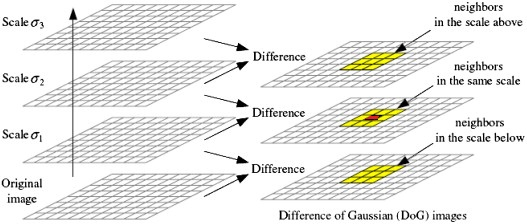
\includegraphics[height=5cm]{DoG.png}
	\caption{多尺度DoG}
\end{figure}\par
标记红色当前像素点,黄色的圈标记邻接像素点,用这个方式,最多检测相邻尺度的26个像素点。如果它是所有邻接像素点的最大值或最小值点,则标记红色被标记为特征点,如此依次进行,则可以完成图像的特征点提取。
因此根据图\ref{differentsigma},遍历图中每一个像素点,可以得到:
\begin{figure}[H]
	\centering
	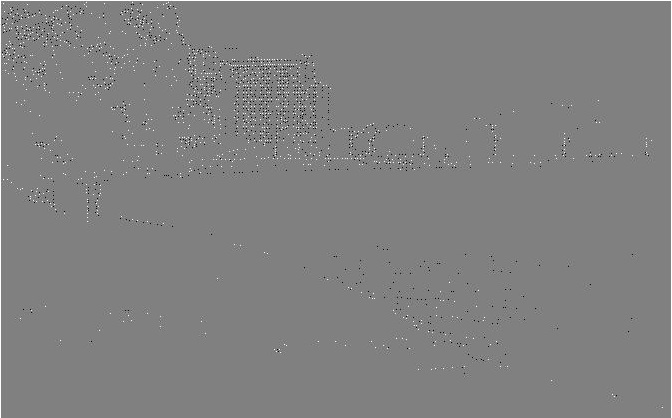
\includegraphics[height=5cm]{DoG4}
	\caption{黑色为极小值,白色为极大值}
\end{figure}\par
最后为了避免重复检测要进行非极大值抑制,把相邻的特征点进行删除,仅保留局部最大值。在原始图像上显示的DoG角点检测结果,如下图所示:
\begin{figure}
	\centering
	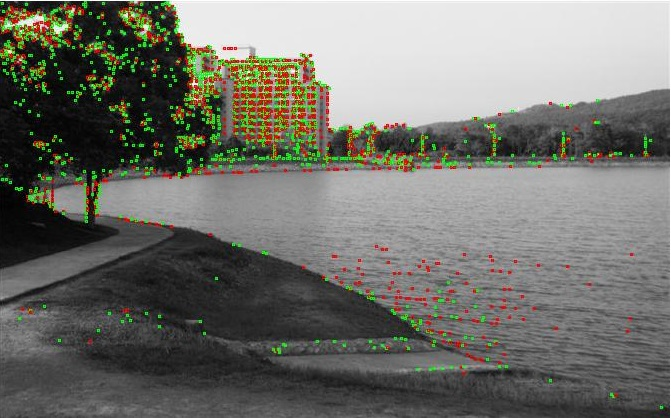
\includegraphics[height=5cm]{DoG5}
	\caption{DoG角点}
\end{figure}
\subsection{快速特征点检测方法}
\subsubsection{FAST特征点}
FAST特征点(Feature from Accelerate Segment Test)\cite{rosten2005fusing}是一种十分快速的特征点检测方法,速度是DoG的100倍。FAST特征点的检测方法很简单,就是检测局部像素灰度值变化来确认特征点的位置。\par
\begin{figure}[H]
	\centering
	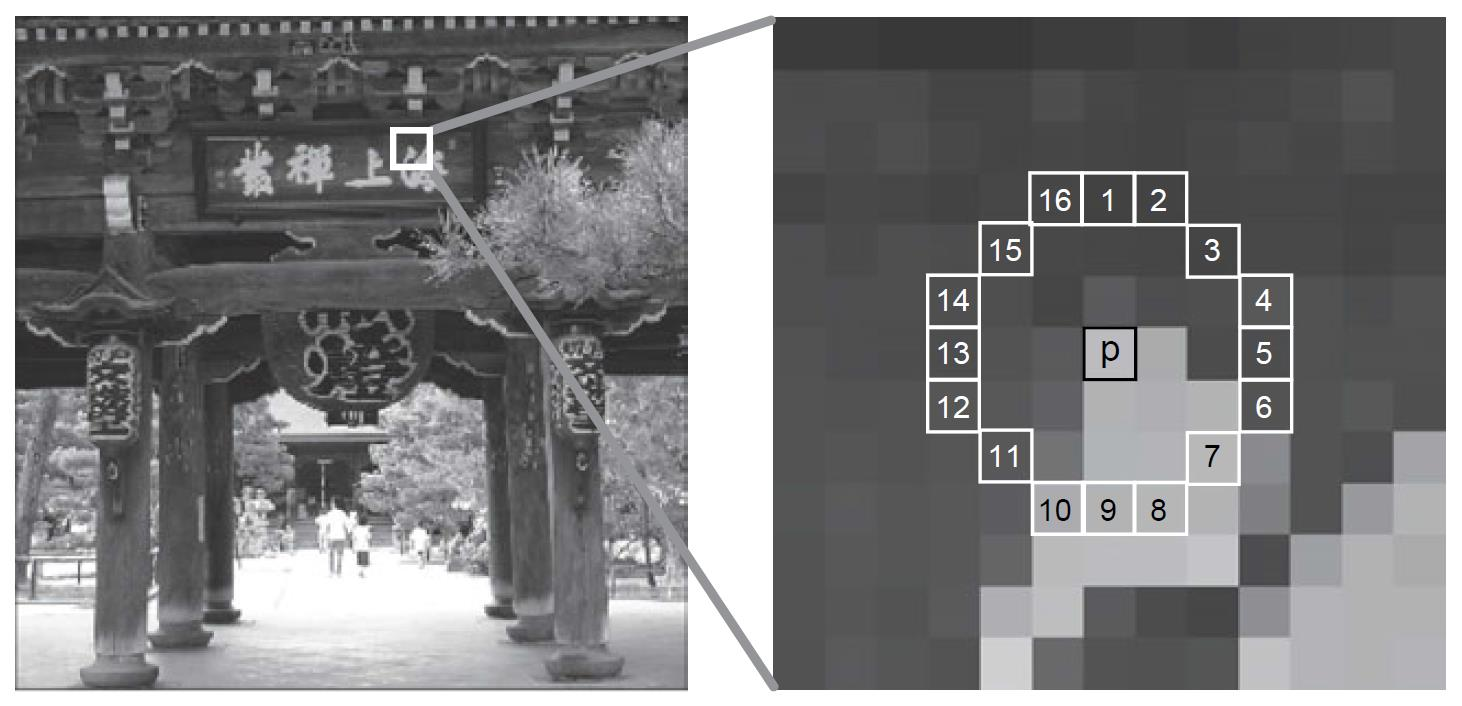
\includegraphics[height=5cm]{FAST}
	\caption{FAST检测原理}
\end{figure}
当有n个像素灰度值明显大于或者小于候选点的时候,该点被认为是特征点。\par
根据n的取值,这些特征点被叫做FAST-n特征点,n一般取9-12。
\subsubsection{ORB特征点}
ORB特征点(Oriented FAST),是用来弥补FAST特征点不具有尺度变性和旋转不变性而设计出来的特征点。事实上ORB特征点也是现阶段SLAM最经常使用的特征点。为了解决尺度不变性,我们可以构造多尺度的图像,在每一层上都进行检测。而对于旋转不变性,我们将在下一节从特征点描述子入手来解决旋转不变性的问题。
\section{特征描述子}
\subsection{描述子的要求}
上一节说明了如何去提取特征点,但是在图像处理过程中提取特征点之后还需要对特征点进行描述。特征描述子就好像是特征点的ID一样。即便在两幅图像中,如果两个特征点的描述子很接近,我们就有一定的把握说这两个特征点是现实空间中的同一个点。这就对描述子有以下几个要求:
\begin{itemize}
	\item 同一个空间点在不同视角的特征点具有高度相似的描述子
	\item 不同的描述子之间差异性应该尽量的大
	\item 描述子需要是一个具有固定长度的向量
	\item 一定的鲁棒性,在不同光照,不同角度下描述子应该相似
\end{itemize}
\subsection{支撑区域与主方向}
某个特征点的描述子计算需要有一个支撑区域,描述子就是根据这个支持区域来计算的。支持区域可以是正方形的,也可以是长方形的。对于较大的图片我们可以采用较大的支持区域,反之亦然。不同大小的支持区域实际上也反映了一个尺度的变化。\par
常见的例如BRIEF是一种二进制描述子,其描述向量由许多0和1组成,这里的0和1编码了关键点附近两个像素的大小关系。如果我们取了256组点,最后就得到了256维由0、1组成的向量。BRIEF是随机选点的,速度非常快,而且由于使用了二进制表达,存储也十分的方便。但是这样的描述子是不具有旋转不变性的,事实上,由于其极快的速度,目前许多SLAM系统中采用的就是添加了角度信息的BRIEF描述子。我们在计算描述子的同时,还通过特征点获得到了它的主方向,大概理解就是支撑区域中每个像素的梯度方向的一个加权和。主方向描述了支撑区域中大多数点的一个梯度方向。因此在计算描述子的时候,我们可以先将主方向旋转到水平方向,然后再进行计算,这样我们计算到的描述子就具有了旋转不变性。
\begin{figure}[H]
	\centering
	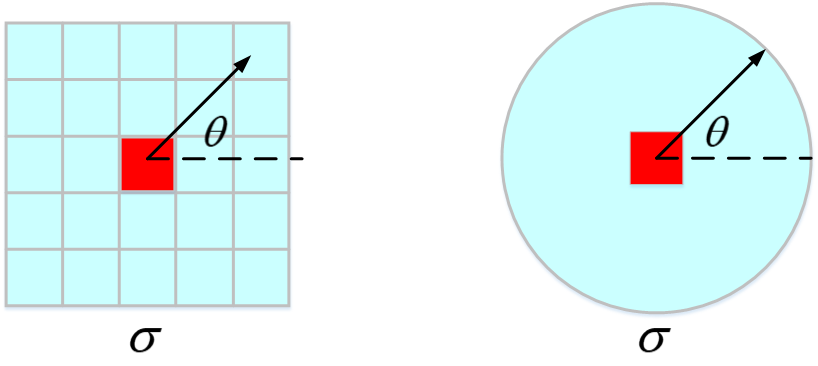
\includegraphics[height=5cm]{zhichiquyu}
	\caption{描述子支撑区域及主方向}
\end{figure}
\subsection{光度一致性}
为了让描述子在不同的光照条件下都有较好的表现,我们通过将图像像素值进行归一化处理,去除光度变化。
\begin{equation}
I^{\prime}=\frac{I-u}{s}
\end{equation}\par
为了解决尺度不变性,我们引入了支撑区域;为了解决旋转不变性,我们将图像主方向旋转至水平;为了解决光照一致性,我们将图像归一化。经过这几个步骤,我们就能过获得一个良好的描述子了。表\ref{descriptors}列出了几种常见的描述子。
\begin{table}[htbp]
	\caption{常见描述子}
	\label{descriptors}
	\begin{tabular}{p{0.16\textwidth}<{\centering} p{0.28\textwidth}<{\centering} p{0.28\textwidth}<{\centering} p{0.28\textwidth}<{\centering}}
		\toprule
		\multicolumn{1}{c}{} & SIFT                                         & SURF                                              & BRIEF                                                \\ \midrule
		确定主方向                & 支撑区域梯度直方图最值方向                                & 支撑区域对Haar算子响应最大方向                                 & 无                                                    \\ \midrule
		确定尺度                 & 建立尺度空间,尺度空间中DoG最值所在的尺度即为特征尺度                 & 尺度空间中Hessian矩阵行列式最值所在的尺度即为特征尺度                    & 无                                                    \\ \midrule
		描述方法                 & 取一正方形支撑区域,分为4×4个子区域,每个区域用8方向的梯度表示每个子区域,共128维 & 同样取4×4个子区域,分别在x,y方向计算Haar算子响应值之和和绝对值之和,4个值描述,共64维 & 在特征点周围随机抽取点对并灰度值大小,根据结果记作0或1,取256组组成256位的二进制串 \\ \bottomrule
	\end{tabular}
\end{table}
\section{特征点匹配}
考虑这样一个问题:对于一个场景,我们在两个不同的角度进行拍摄得到两张照片。对这两张照片提取特征点之后如何去判断哪两个特征点描述的是空间中的同一个点呢?这就引出了特征点匹配问题。前面说了,特征点的描述子就像特征点的ID一样,我们希望不管这个点在什么条件下,总是能被人们检测出这就是那个点。我们可以这样认为:一个设计良好的描述子,它在不同视角下的距离应该是差不多的。\par
\begin{figure}[H]
	\centering
	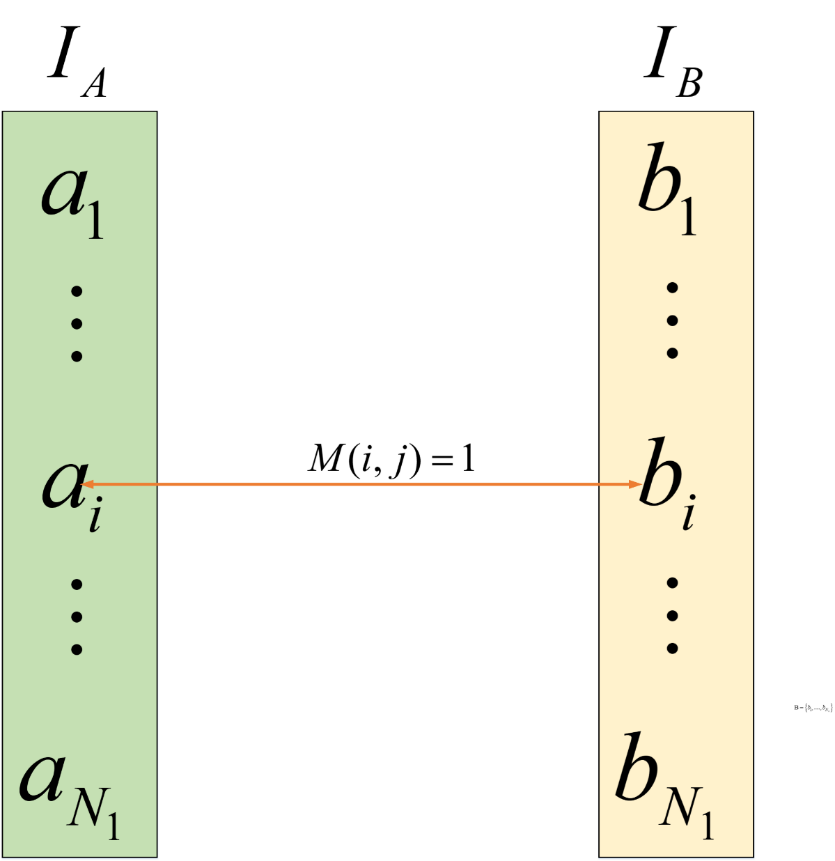
\includegraphics[height=5cm]{tezhengdianjuli}
	\caption{特征点A和B的描述子}
\end{figure}
我们有很多种方法可以度量两个描述子是否接近:
\begin{table}[htb]
	\centering
	\caption{度量距离的几种方法}
	\begin{tabular}{ll}
		\toprule
		距离 & 公式\\
		\midrule
		欧式距离 & $D_{e u c}(\boldsymbol{a}, \boldsymbol{b})=\|\boldsymbol{a}-\boldsymbol{b}\|_{2}=\left(\sum_{i=1}^{n}\left(a_{i}-b_{i}\right)^{2}\right)^{\frac{1}{2}}$ \\
		马氏距离 & $D_{\text {mahal}}(\boldsymbol{a}, \boldsymbol{b})=\left((\boldsymbol{a}-\boldsymbol{b})^{T} \Sigma^{-1}(\boldsymbol{a}-\boldsymbol{b})\right)^{\frac{1}{2}}$   \\
		归一化互相关 & $N C C(\boldsymbol{a}, \boldsymbol{b})=\sum_{i=1}^{n} \frac{1}{s_{a} s_{b}}\left(a_{i}-u_{a}\right)\left(b_{i}-u_{b}\right)$       \\
		汉明距离 & $D_{h a m}(\boldsymbol{a}, \boldsymbol{b})=\sum_{i=1}^{n} a_{i} \oplus b_{i}$\\
		\bottomrule	
	\end{tabular}
  \note{注:$a_{i} \oplus b_{i}$即两者相同时为1,不同为0}
\end{table}
\subsection{匹配策略}
特征的匹配是针对特征描述子的进行的,上面提到特征描述子通常是一个向量,两个特征描述子的之间的距离可以反应出其相似的程度,也就是这两个特征点是不是同一个。根据描述子的不同,可以选择不同的距离度量。如果是浮点类型的描述子,可以使用其欧式距离;对于二进制的描述子(BRIEF)可以使用其汉明距离。\par
\subsubsection{Lowe’s algorithm}
有了计算描述子相似度的方法,那么在特征点的集合中如何寻找和其最相似的特征点,这就是特征点的匹配了。最简单直观的方法就是暴力匹配方法(Brute-Force Matcher),计算某一个特征点描述子与其他所有特征点描述子之间的距离。\par
然后将得到的距离进行排序,取距离最近的一个作为匹配点。这种方法简单粗暴,其结果也是显而易见的,通过上面的匹配结果,也可以看出有大量的错误匹配,这就需要使用一些机制来过滤掉错误的匹配。\par
Lowe's algorithm\cite{muja2009fast}是我们常用的过滤掉错误匹配点的方法。它的原理也很简单,对于一幅图中的特征点,找到另一幅图中和它欧氏距离最近的两个特征点,如果最邻近距离除以次临近距离的值小于某个阈值,则说明最邻近点相比于次临近点足够优秀,就认为这一对点是一组匹配,反之则不是。如图\ref{lowe's filter}所示,可以显然看到经过过滤之后匹配的点已经很准确了。
\begin{figure}[H]
	\centering
	\begin{subfigure}[ht]{0.4\textwidth}
		\centering
		\includegraphics[height=4cm]{matches}
		\caption{BFMatcher结果}
		\label{no filter}
	\end{subfigure}
	\quad
	\begin{subfigure}[ht]{0.4\textwidth}
		\centering
		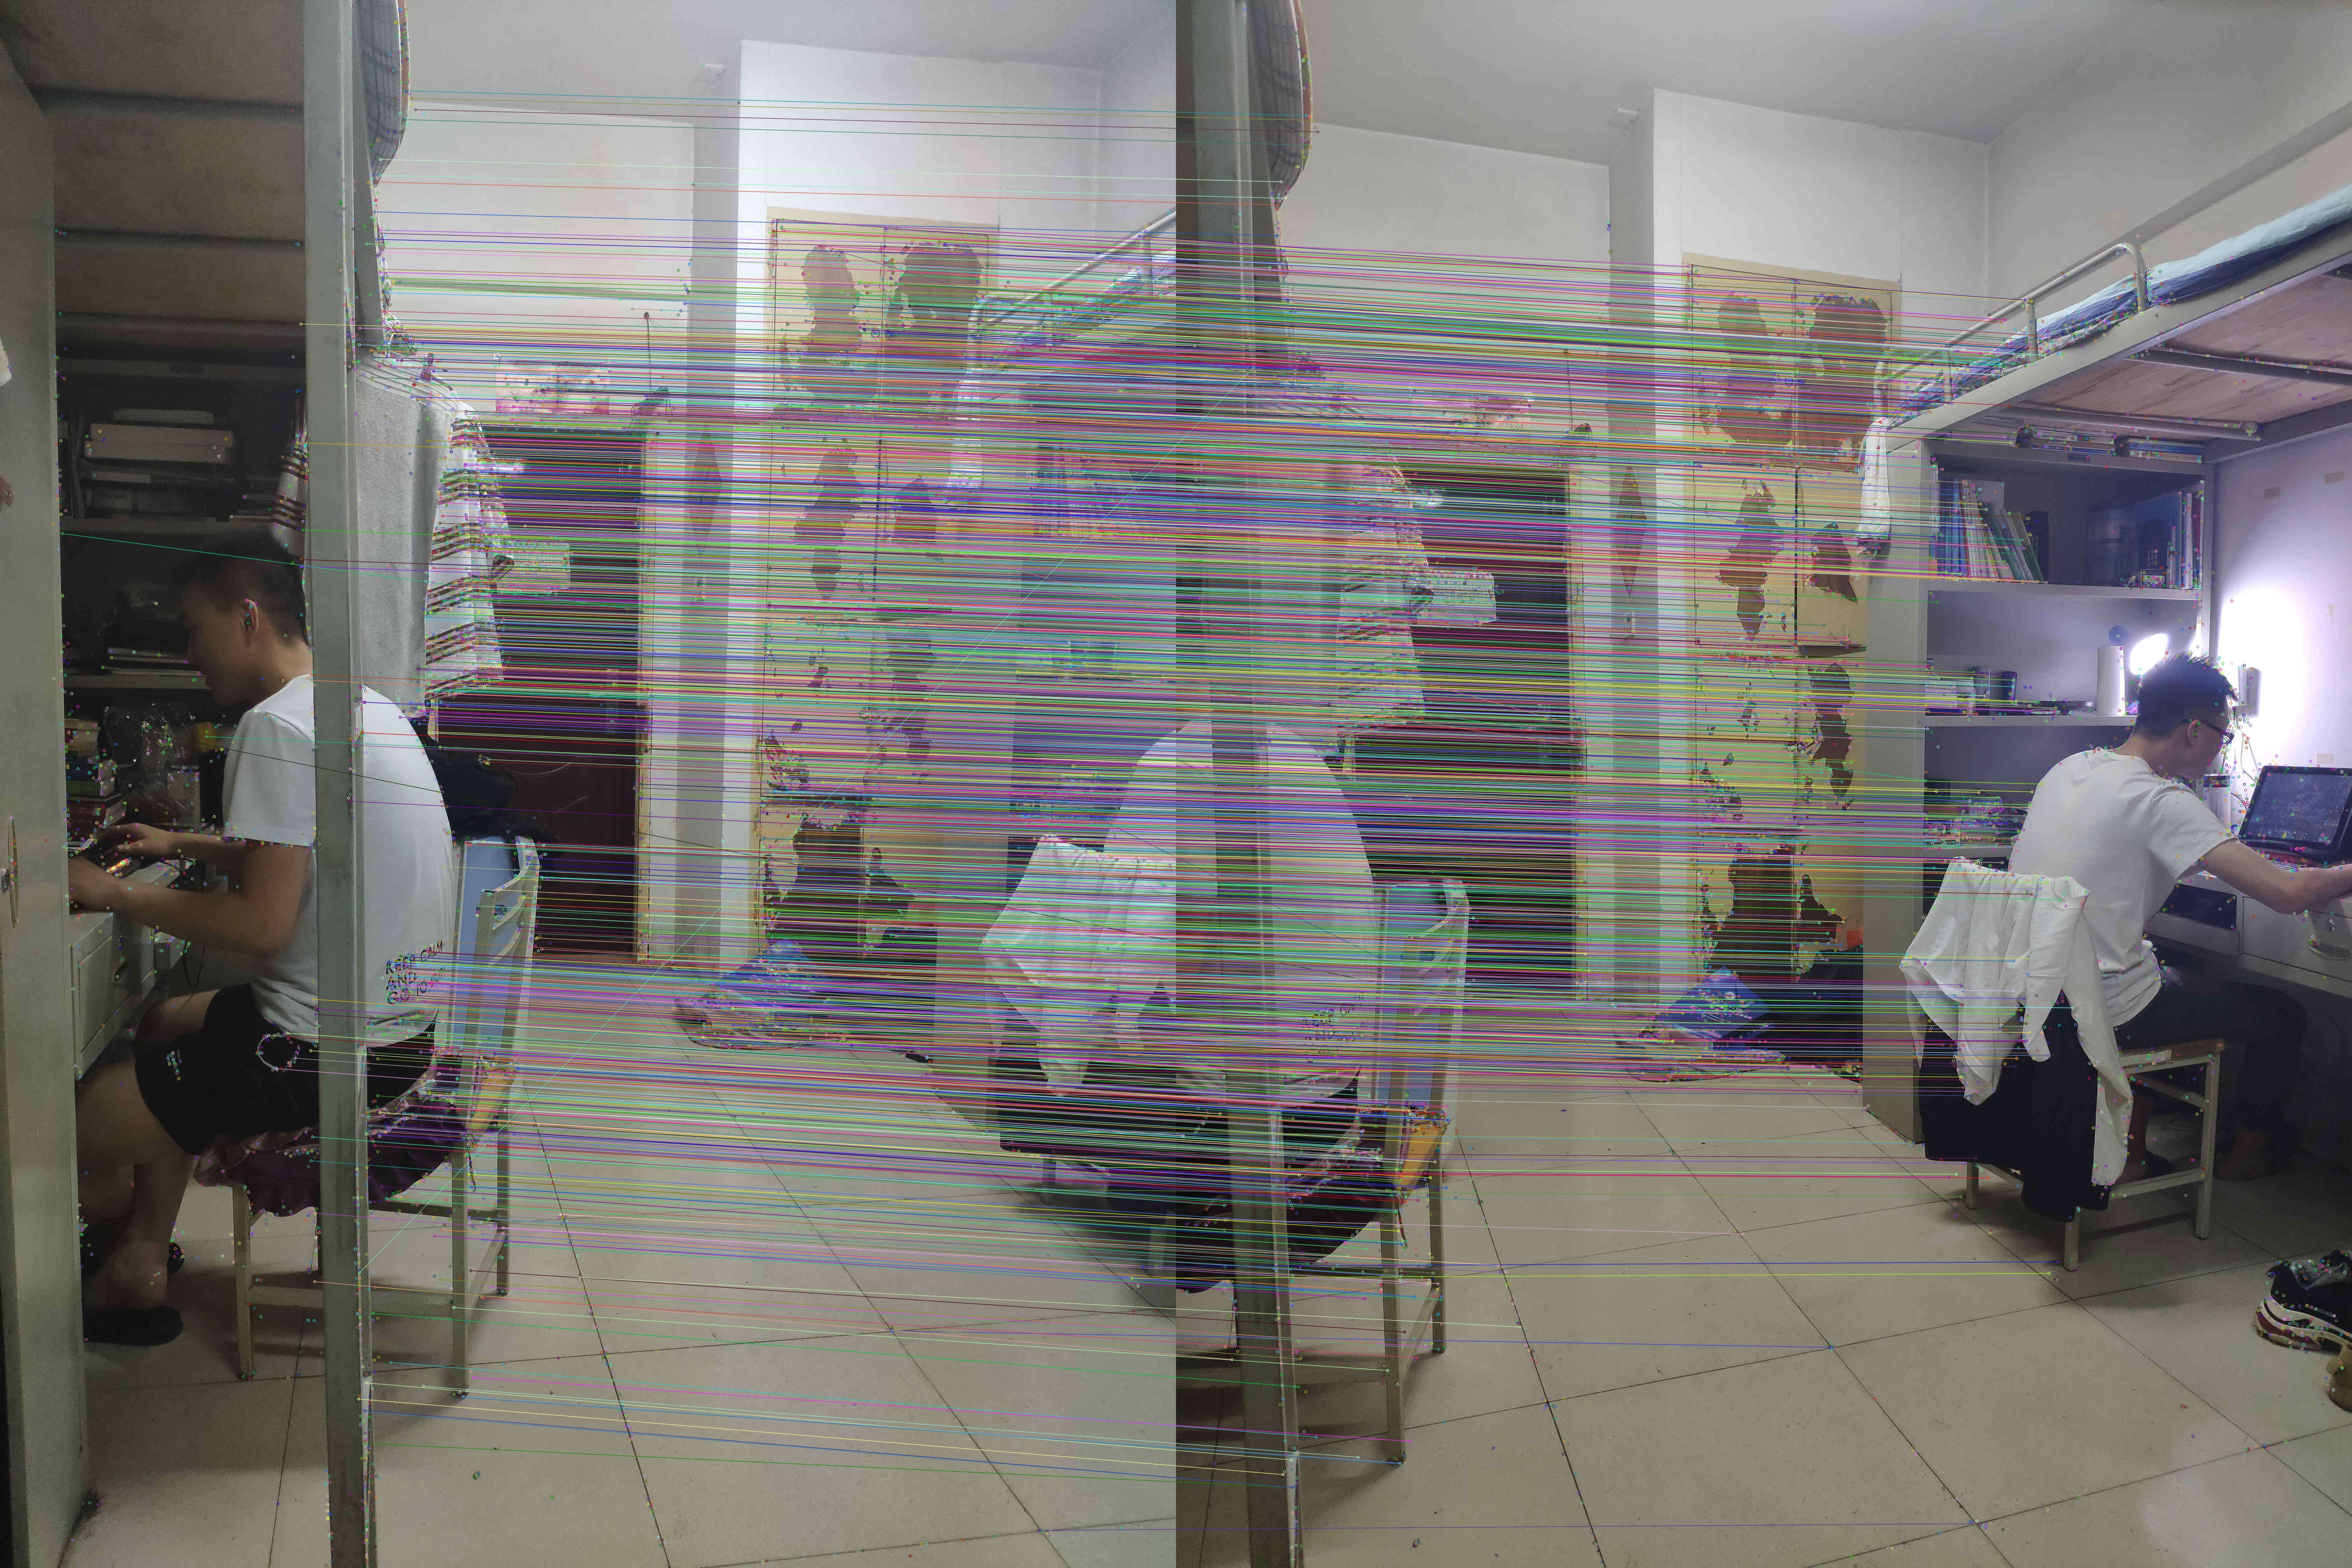
\includegraphics[height=4cm]{matches1}
		\subcaption{Lowe‘s算法过滤}
		\label{lowe's filter}
	\end{subfigure}\\
	\begin{subfigure}[ht]{0.4\textwidth}
		\centering
		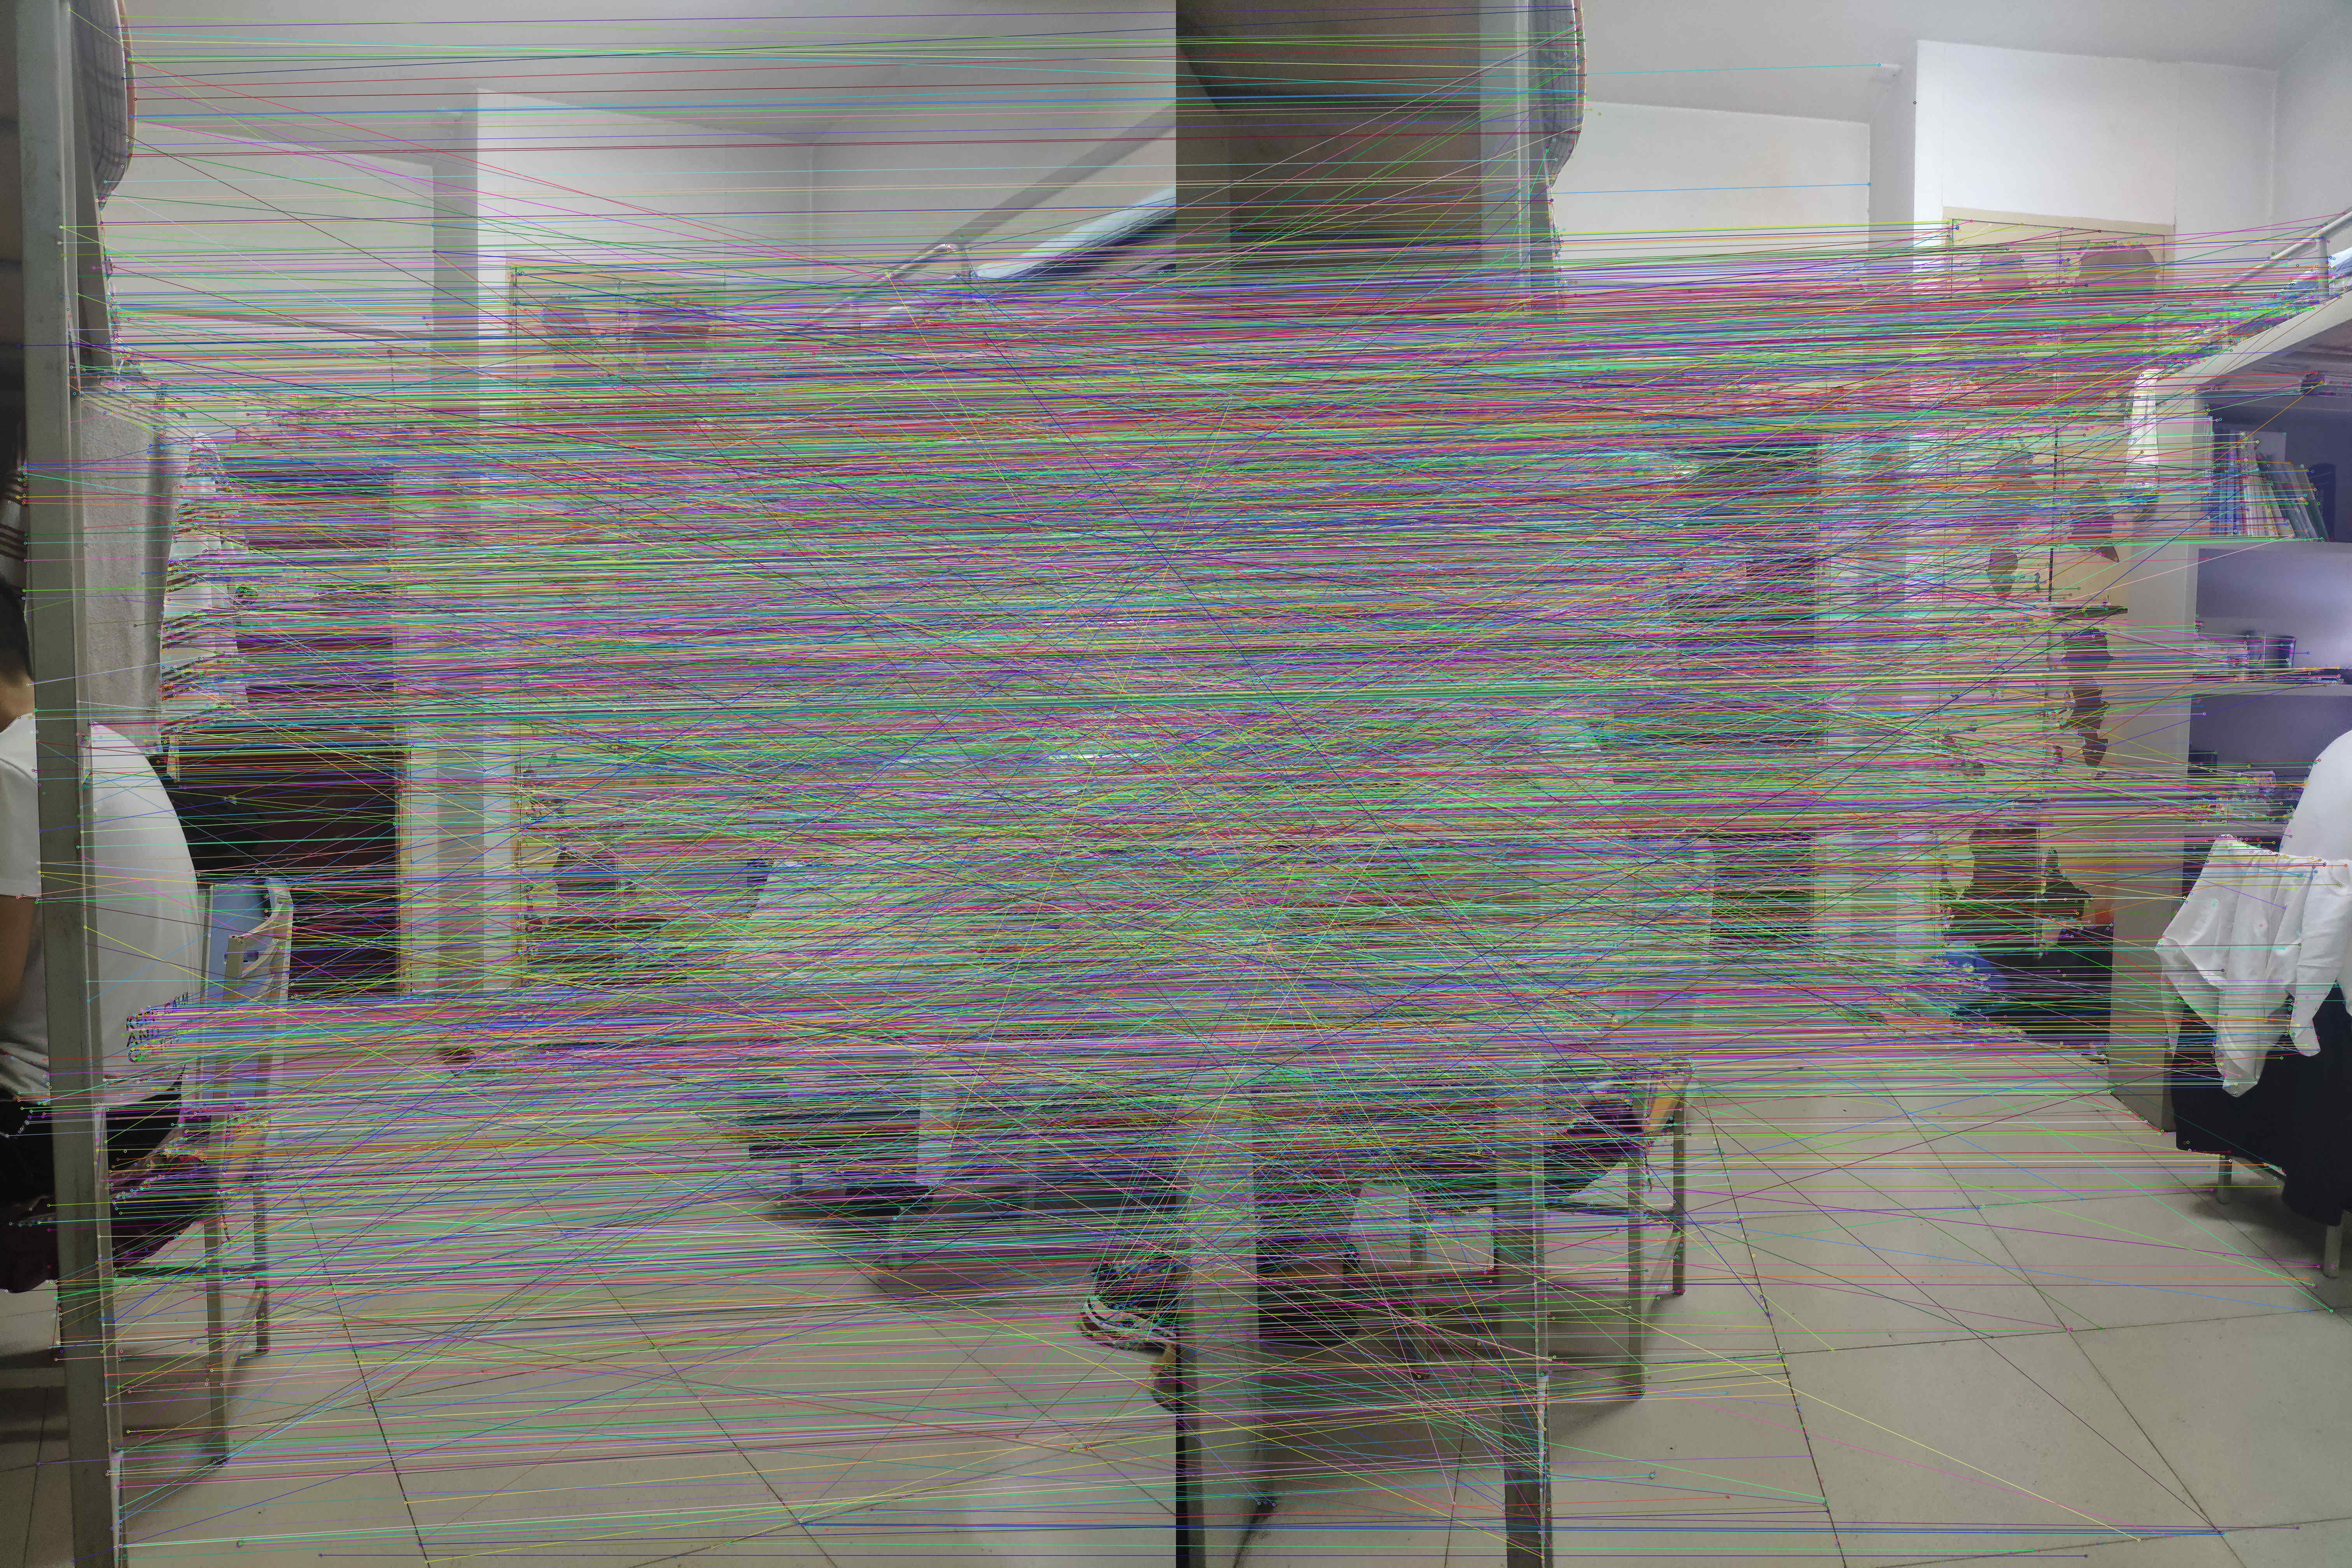
\includegraphics[height=4cm]{matches2}
		\caption{交叉过滤结果}
		\label{crosscheck filter}
	\end{subfigure}
	\quad
	\begin{subfigure}[ht]{0.4\textwidth}
		\centering
		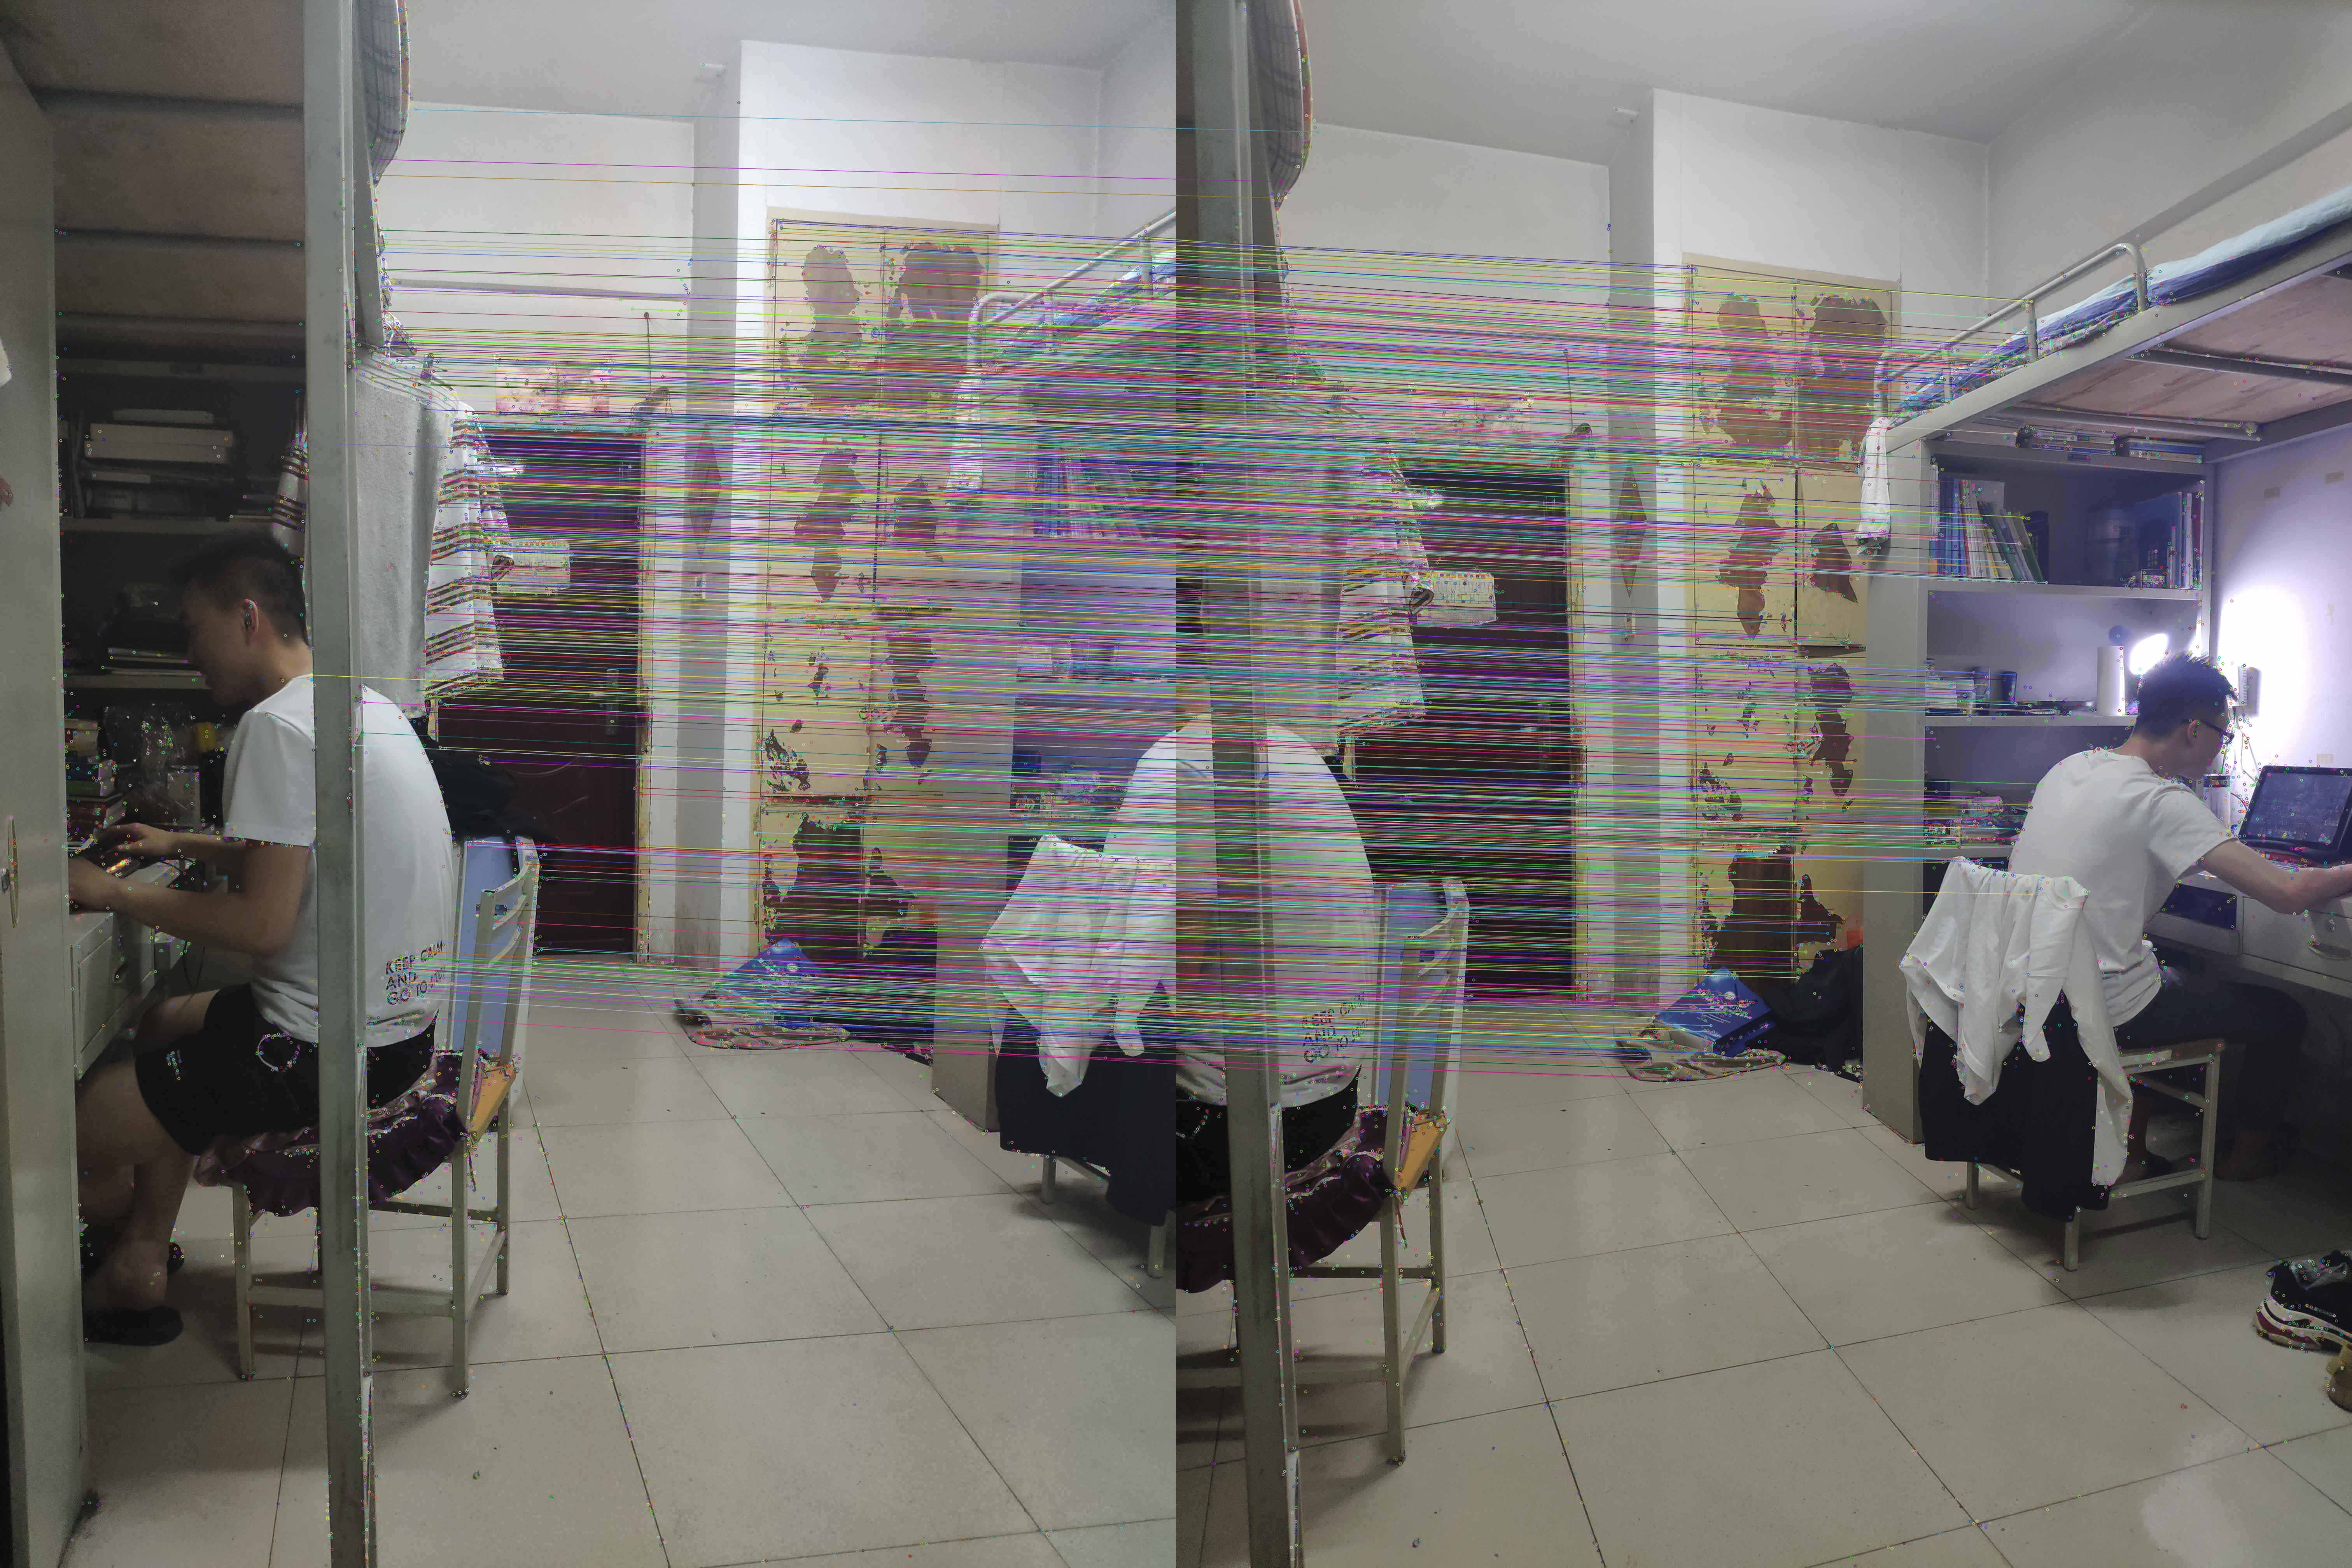
\includegraphics[height=4cm]{matches3}
		\subcaption{RANSAC算法过滤}
		\label{RANSAC filter}
	\end{subfigure}
	\caption{匹配过程}
	\label{filters}
\end{figure}
\subsubsection{交叉匹配}
交叉过滤基于这样一个简单的设想:如果特征点A认为B是它的最优匹配,那么相应的,特征点B也应该认为特征点A是它的最优匹配。具体操作的话就是再进行一次匹配,反过来使用被匹配到的点进行匹配,如果匹配到的仍然是第一次匹配的点的话,就认为这是一个正确的匹配。假如第一次特征点A使用暴力匹配的方法匹配到特征点B;反过来,使用特征点B进行匹配,如果匹配到的仍然是特征点A,则就认为这是一个正确的匹配,否则就是一个错误的匹配。对比图\ref{no filter}和图\ref{crosscheck filter},虽然不能明显的看出来差别,但是根据定量测试来看,交叉匹配能够使\ref{no filter}中7966个匹配降低至5091个匹配。
\subsubsection{RANSAC方法}
RANSAC算法的基本假设是样本中包含正确数据(inliers,可以被模型描述的数据),也包含异常数据(outliers,偏离正常范围很远、无法适应数学模型的数据),即数据集中含有噪声。这些异常数据可能是由于错误的测量、错误的假设、错误的计算等产生的。同时RANSAC也假设,给定一组正确的数据,存在可以计算出符合这些数据的模型参数的方法。因此,我们可以利用RANSAC方法去不断估计两张图之间的单应矩阵或者基础矩阵来获得过滤出inliers。
\begin{algorithm}[htb]
	\KwIn{\\
	data – 所有的匹配\quad
	model – 单应矩阵\\
	k – 算法迭代次数\quad
	t – 投影误差阈值\\
}
	\SetAlgoLined
	\KwResult{bestModel – 单应矩阵 \quad inliers – 内点	}
	\KwData{bestModel $\leftarrow$ NULL \quad bestInliers $\leftarrow$ 0\;}

	\For{iteration$\leftarrow$0 to k}{
		maybeInliers$\leftarrow$随机抽取四个不共线的点\;
		maybeModel$\leftarrow$从maybeInliers中计算单应矩阵\;
		newInliers$\leftarrow$$\emptyset$\;
		\For{each match $\in$ data}{
			error$\leftarrow$计算match点对的重投影误差\;
			\If{error < t}{将该match添加进newInliers}	
	}
		\If{newInliers的元素数目 > bestInliers元素数目}{
			bestInliers$\leftarrow$newInliers+maybeInliers\;
			bestModel$\leftarrow$maybeModel
		}
	}
	\caption{RANSAC算法}
	\label{algo:RANSAC}
\end{algorithm}
\par
事实上,根据测试结果来看,选用单应矩阵作为RANSAC的模型并不合适。查阅资料得知单应矩阵假设所有点都位于同一个平面上,显然宿舍这样的场景并不适合单应矩阵。图\ref{RANSAC filter}的结果是通过另外一个矩阵——基础矩阵计算得来的。至于什么是单应矩阵,什么是基础矩阵,会在下一章作介绍。













% !TeX root = ../main.tex
\chapter{对极几何}
通过上一章的介绍,我们知道了如何在一张图中的提取出特征点和对应的描述子,并通过描述子的匹配来获取两张图片特征点的对应关系。在上一章的最后我们提到了基础矩阵和单应矩阵,它们都属于对极几何的范畴,这一章就来介绍一下对极几何。
\section{对极约束}
立体成像的基本几何就是对极几何。图\ref{epipolargeometry}是最经典的对极几何示意图。$O_1$和$O_2$为两个相机(也有可能是一个相机在不同时刻的位置)的位置,P为空间中一点,两个相对的白色平面是归一化平面。$p_1$和$p_2$是P点在归一化平面上的对应点,$e_1$,$e_2$为归一化平面和$O_1$,$O_2$的交点。$O_1$$O_2$为基线,也被称作相机的移动方向。\par
\begin{figure}[H]
	\centering
	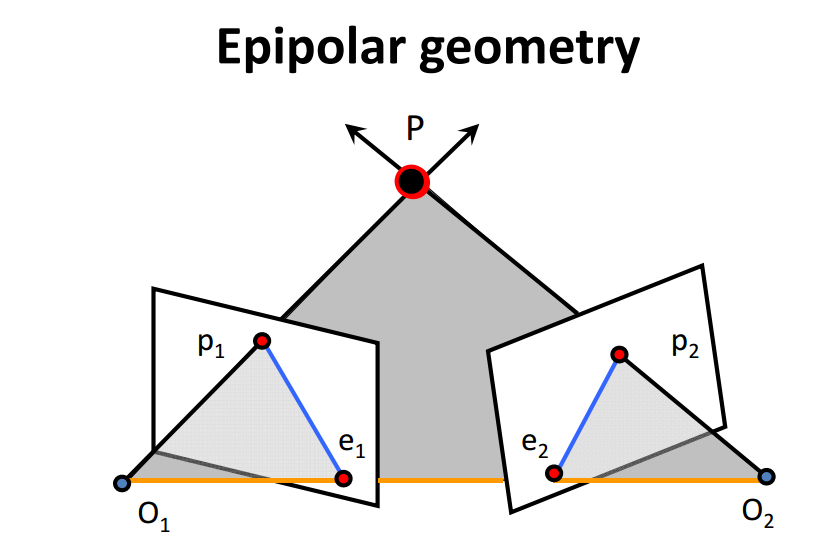
\includegraphics[height=5cm]{epipolargeometry}
	\caption{对极几何}
	\label{epipolargeometry}
\end{figure}
这里介绍几个对极几何中常用的概念: $e_1$和$e_2$被称作极点,P$O_1$$O_2$平面为极面,$p_1$$e_1$为极线,同理$p_2$$e_2$也为极线。
所谓对极约束,指的就是相机$O_1,O_2,\text{点}P$在同一个平面上。也就是向量$\overrightarrow{O_1O_2},\overrightarrow{O_1P},\overrightarrow{O_2P}$共面,即三者混合积为0:
\begin{equation}
\overrightarrow{O_1P}\cdot\left[\overrightarrow{O_1O_2}\times\overrightarrow{O_2P} \right]=0
\end{equation}
设相机$O_2$相对于相机$O_1$的旋转为R,位移为t,向量$\overrightarrow{O_1p_1}$为$\vec{x}$($O_1$坐标系下),向量$\overrightarrow{O_2p_2}$为$\vec{x^\prime}$($O_2$坐标系下),两相机的内参是$K_1,K_2$,由相机成像原理知:
\begin{equation}
\begin{aligned}
	d_{1} \boldsymbol{x}_{1}=&\boldsymbol{K}_{1} \boldsymbol{P}\\
	d_{2} \boldsymbol{x}_{2}=&\boldsymbol{K}_{2}(\boldsymbol{R P}+\boldsymbol{t})
\end{aligned}
\end{equation}
联立上式得:
\begin{equation}
d_{2} \boldsymbol{K}_{2}^{-1} \boldsymbol{x}_{2}=d_{1}\boldsymbol{R} \boldsymbol{K}_{1}^{-1} \boldsymbol{x}_{1}+\boldsymbol{t}
\end{equation}
两边同时叉乘t\footnote{$\mathbf{a} \times \mathbf{b}=\left[ \begin{array}{ccc}{0} & {-a_{z}} & {a_{y}} \\ {a_{z}} & {0} & {-a_{x}} \\ {-a_{y}} & {a_{x}} & {0}\end{array}\right] \left[ \begin{array}{l}{b_{x}} \\ {b_{y}} \\ {b_{z}}\end{array}\right]=\left[ \mathbf{a}\right]_{\times}\mathbf{b}$}:
\begin{equation}
d_{2} \left[\boldsymbol{t}\right]_{\times}\boldsymbol{K}_{2}^{-1} \boldsymbol{x}_{2}=d_{1}\left[\boldsymbol{t}\right]_{\times}\boldsymbol{R} \boldsymbol{K}_{1}^{-1} \boldsymbol{x}_{1}
\end{equation}
再同时左乘$\left(\boldsymbol{K}_{2}^{-1} \boldsymbol{x}_{2}\right)^T$:
\begin{equation}
\boldsymbol{x}_{2}^T\boldsymbol{K}_{2}^{-T} \left[\boldsymbol{t}\right]_{\times}\boldsymbol{R} \boldsymbol{K}_{1}^{-1} \boldsymbol{x}_{1}=0
\end{equation}
若令$\boldsymbol{K}_{1}^{-1} \boldsymbol{x}_{1}=\hat{\boldsymbol{x}}_1,\boldsymbol{K}_{2}^{-1} \boldsymbol{x}_{2}=\hat{\boldsymbol{x}}_2$,也就是$\hat{\boldsymbol{x}}_1,\hat{\boldsymbol{x}}_2$分别为归一化平面坐标,则:
\begin{equation}
\hat{\boldsymbol{x}}_2^T\left[\boldsymbol{t}\right]_{\times}\boldsymbol{R}\hat{\boldsymbol{x}}_1=0
\end{equation}
我们称本质矩阵$\boldsymbol{E}=[\boldsymbol{t}]_{\times} \boldsymbol{R}$,基础矩阵$\boldsymbol{F}=\boldsymbol{K}_{2}^{-T} \boldsymbol{E} \boldsymbol{K}_{1}^{-1}$\par
\section{基础矩阵}
可以看到,我们之所以要求解本质矩阵或者基础矩阵,是因为它们包含着图像之间的运动信息,只要求得本质矩阵,就能够从中分解除R和t,那么相机的运动信息也就清楚了。想要求解本质矩阵,首先要求解基础矩阵,然后去掉内参信息就能得到本质矩阵。求解基础矩阵我们一般有以下方法。
\subsection{直接线性变换法}
对于一对匹配点$\boldsymbol{x}_{1}=\left[ u_{1},v_{1},1\right]^{\mathrm{T}}, \boldsymbol{x}_{2}=\left[ u_{2},v_{2},1\right]^{\mathrm{T}}$根据对极约束$\boldsymbol{x}_{2}^{T} \boldsymbol{F x}_{1}=\mathbf{0}$:
\begin{equation}
\left( \begin{array}{ccc}{u_{1}} & {v_{1}} & {1}\end{array}\right) \left[ \begin{array}{ccc}{F_{11}} & {F_{12}} & {F_{13}} \\ {F_{21}} & {F_{22}} & {F_{23}} \\ {F_{31}} & {F_{32}} & {F_{33}}\end{array}\right] \left( \begin{array}{l}{u_{2}} \\ {v_{2}} \\ {1}\end{array}\right)=0
\end{equation}
令$f=\left[ F_{11},F_{12},F_{13},F_{21},F_{22},F_{23},F_{31},F_{32},F_{33} \right]^{T}$则有:
\begin{equation}
\left[
{u_{1} u_{1},}{u_{1} v_{2},}{u_{1},}{v_{2} u_{1},}{v_{1} v_{2},}{v_{1},}{u_{2},}{v_{2},}{1}
\right] f=0
\end{equation}
当有n对匹配点时:
\begin{equation}
\boldsymbol{A}=
\left\lbrace
	\begin{array}{c}
	u_{1}^{(1)} u_{1}^{(1)}, u_{1}^{(1)} v_{2}^{(1)}, u_{1}^{(1)},  v_{1}^{(1)} u_{2}^{(1)}, v_{1}^{(1)} v_{2}^{(1)}, v_{1}^{(1)}, u_{2}^{(1)}, v_{2}^{(1)},1\\
	u_{1}^{(2)} u_{1}^{(2)}, u_{1}^{(2)} v_{2}^{(2)}, u_{1}^{(2)},  v_{1}^{(2)} u_{2}^{(2)}, v_{1}^{(2)} v_{2}^{(2)}, v_{1}^{(2)}, u_{2}^{(2)}, v_{2}^{(2)},1\\
	\cdots\\
	u_{1}^{(n)} u_{1}^{(n)}, u_{1}^{(n)} v_{2}^{(n)}, u_{1}^{(n)},  v_{1}^{(n)} u_{2}^{(n)}, v_{1}^{(n)} v_{2}^{(n)}, v_{1}^{(n)}, u_{2}^{(n)}, v_{2}^{(n)},1\\
	\end{array}
\right\rbrace 
\end{equation}
即$\boldsymbol{A}f=0$。
要保证有唯一解至少需要8对匹配点,当匹配点n=8时,若A非奇异,则有唯一解,称为8点法\cite{longuet1981computer}。若n>8,则可用最小二乘解,也就是$\boldsymbol{A}^T\boldsymbol{A}$的最小特征值对应的特征向量即为最优解。
\subsection{RANSAC法}
RANSAC方法的思想我们在上一章已经介绍过了,应用RANSAC法求解基础矩阵也是有以下几个步骤:
\begin{enumerate}
	\item 随机从匹配的点对中选择8个点,使用8点法估算出基础矩阵$F_i$
	\item 计算其余的点对到其对应对极线的距离$d_n$,如果$d_n≤d$则该点为内点,否则为外点。记下符合该条件的内点的个数为$m_i$
	\item 迭代k次,或者某次得到内点的数目$m_i$占有的比例大于等于95\%,则停止。选择$m_i$最大的基础矩阵作为最终的结果。
\end{enumerate}\par
RANSAC能够不依赖于任何额外信息的情况下,将数据划分为内点和外点。但也有其相应的缺点,RANSAC并不能保证得到正确的结果,需要提高迭代的次数;另一个是,内点外点的判断需要设置阈值。\par
阈值的大小设置也是有技巧的,对于不同图片大小,需要设置不同的阈值。事实上经过实验,采用归一化平面坐标而不是像素坐标来计算基础矩阵会有较好的结果。
\section{单应矩阵}
除了基础矩阵和本质矩阵,还有单应矩阵(Homography)$\boldsymbol{H}$,它主要适用于特征点都位于同一个平面上的情况。比如两个相机都拍摄一面纹理丰富的墙,这就是单应矩阵大展身手的时候。下面我们来大概介绍一下单应矩阵\par
\begin{figure}[H]
	\centering
	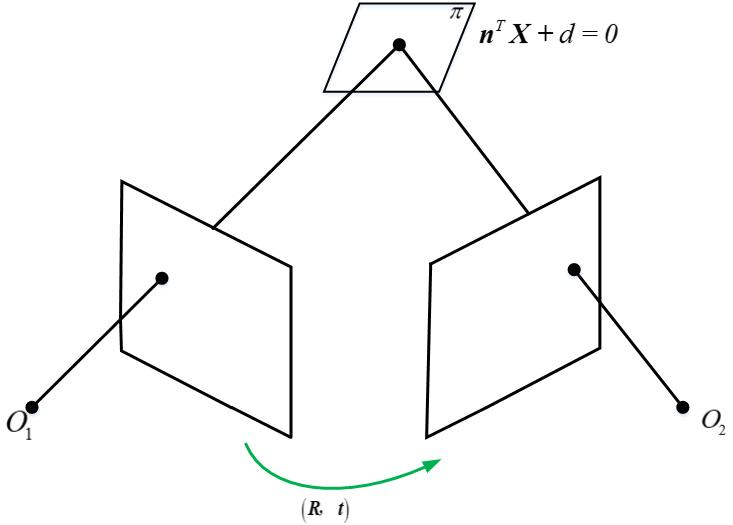
\includegraphics[height=5cm]{homography}
	\caption{单应矩阵条件}
\end{figure}
设特征点所在的平面方程为:
\begin{equation}
	\boldsymbol{n}^{T} \boldsymbol{P}+d=0 \Rightarrow -\frac{\boldsymbol{n}^{T} \boldsymbol{P}}{d}=1
\end{equation}
故:
\begin{equation}
\begin{aligned} x_{2} &=K_{2}(R P+t) \\ &=K_{2}\left(R P+t \cdot\left(-\frac{n^{T} P}{d}\right)\right) \\ &=K_{2}\left(R-\frac{t n^{T}}{d}\right) P \\ &=K_{2}\left(R-\frac{t n^{T}}{d}\right) K_{1}^{-1} x_{1} \end{aligned}
\end{equation}
故:
\begin{equation}
\boldsymbol{x}_{2}=\boldsymbol{H x}_{1}, \quad \boldsymbol{H}=\boldsymbol{K}_{2}\left(\boldsymbol{R}-\frac{\boldsymbol{t} \boldsymbol{n}^{T}}{d}\right) \boldsymbol{K}_{1}^{-1}
\label{homography}
\end{equation}
单应矩阵说明了两个成像平面像素之间的映射关系,从公式\ref{homography}上来看,单应矩阵只和空间平面位置$\boldsymbol{n}$,旋转矩阵R,平移t以及相机内参有关。由于单应矩阵的平面假设,我们常在拍摄对象在平面场景时或者可以假设近似为平面场景时(如无人机俯拍)应用单应矩阵来恢复相机位姿。
\section{相机姿态的恢复}
这里介绍一下如何通过本质矩阵$E$来对相机的位姿$R,t$进行恢复。我们主要用到的方法是SVD分解\cite{multiview}。\par
首先对E进行SVD分解:
\begin{equation}
\boldsymbol{E}=\boldsymbol{U} \Sigma \boldsymbol{V}^{T}, \quad \boldsymbol{\Sigma}=\operatorname{diag}(\sigma, \quad \sigma, \quad 0)
\end{equation}
此时有两个t和两个R都有可能成立
\begin{equation}
\begin{array}{cc}
{t_{1}=U( :, 2)} & {R_{1}=U R_{Z}\left(\frac{\pi}{2}\right) V^{T}} \\
{t_{2}=-U( :, 2)} & {R_{2}=U R_{Z}^{T}\left(\frac{\pi}{2}\right) V^{T}}
\end{array}
\end{equation}
其中:
\begin{equation}
\boldsymbol{R}_{z}\left(\frac{\pi}{2}\right)=\left( \begin{array}{ccc}{0,} & {-1,} & {0} \\ {1,} & {0,} & {0} \\ {0,} & {0,} & {1}\end{array}\right), \boldsymbol{R}_{z}^{T}\left(\frac{\pi}{2}\right)=\left( \begin{array}{ccc}{0,} & {1} & {0} \\ {-1} & {0,} & {0} \\ {0,} & {0,} & {1}\end{array}\right)
\end{equation}
如下图所示,我们得到了四种情况$(t_1,R_1),(t_1,R_2),(t_2,R_1),(t_2,R_2)$。此时,我们只需要验证一下哪一种情况下点P在两个相机的正面。OpenCV已经为我们提供了方便的函数recoverpose()由本质矩阵恢复$R,t$。
\begin{figure}[H]
	\centering
	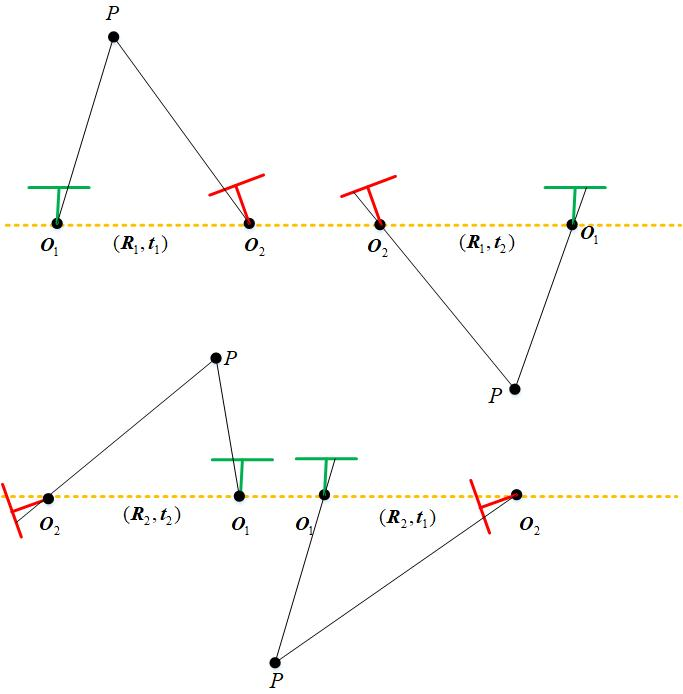
\includegraphics[height=10cm]{svd}
	\caption{四种可能的情况}
\end{figure}























% !TeX root = ../main.tex
\chapter{视觉里程计}
视觉SLAM主要分为视觉前端和后端优化。前端也称为视觉里程计,这是通过相邻图像间的信息估计出粗略的相机运动,给后端提供较好的初始值。视觉里程计的实现也分几种,按照是否需要提取特征,分为特征点法的前端和不提取特征点的直接法前端。基于特征点法的前端被认为是较好的方法,它运行稳定,对光照、动态物体不敏感,是目前比较成熟的解决方案。通过前几章的技术积累,我们已经初步具备了设计一个视觉里程计的能力。\par
\section{单目SLAM的初始化}
对于单目SLAM来说,存在一个尺度问题。我们知道对极几何满足这样的关系:
\begin{equation}
\hat{\boldsymbol{x}}_2^T\left[\boldsymbol{t}\right]_{\times}\boldsymbol{R}\hat{\boldsymbol{x}}_1=0
\end{equation}
可以看到,在方程两边同时乘以某个常数,方程仍然成立。这就意味着从本质矩阵E估计出的t是不可靠的。所以我们并不能连续计算两幅相邻的图片去估计相机的位姿。那解决这个问题的方法就是对前两幅图片的$\boldsymbol{t}$进行归一化,后续的图片通过PnP(后面会介绍)来计算R和t。在单目视觉中,我们对初始两张图像的$\boldsymbol{t}$归一化相当于固定了尺度。虽然我们并不知道$\boldsymbol{t}$的单位是多少,但是我们可以以前两幅图的移动为单位1,以此计算特征点的3D位置。由以上描述我们也可以知道,前两幅图的位置关系不能是纯旋转。纯旋转的两张图无法进行初始化。
\section{三角测量}
\begin{figure}[H]
	\centering
	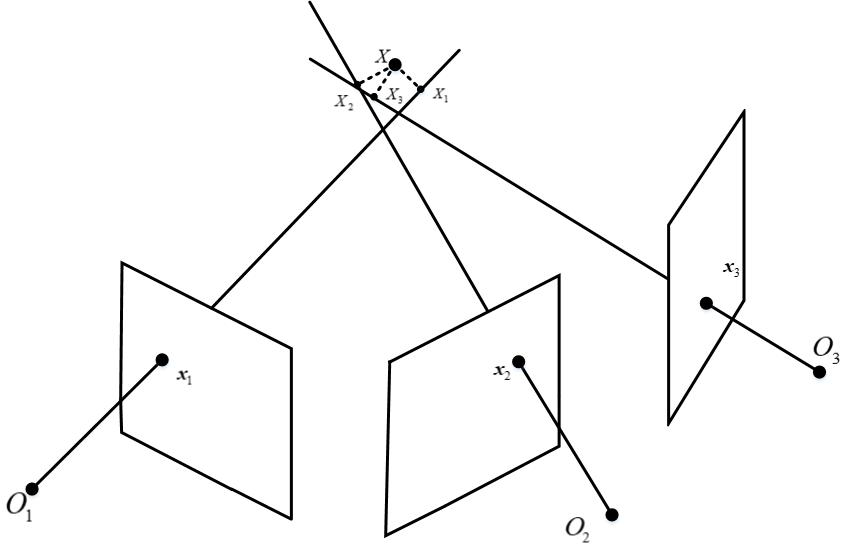
\includegraphics[height=5cm]{triangulation}
	\caption{三角化}
	\label{fig:triangulation}
\end{figure}
假如我们设$x_1,x_2$为两个特征点的归一化坐标,那么他们满足:
\begin{equation}
	s_1\boldsymbol{x_1}=s_2\boldsymbol{Rx_2}+\boldsymbol{t}
\end{equation}
现在我们已经解得$\boldsymbol{R},\boldsymbol{t}$,想要求解出$s_1,s_2$。以求解$s_2$为例,先在两边叉乘一个$x_1$:
\begin{equation}
s_1\left[\boldsymbol{x_1}\right]_{\times}\boldsymbol{x_1}=0=s_2\left[\boldsymbol{x_1}\right]_{\times}\boldsymbol{Rx_2}+\left[\boldsymbol{x_1}\right]_{\times}\boldsymbol{t}
\end{equation}
式子左侧为0,右边的R和t以及$x_1,x_2$都是已知的,由此求得$s_2$。OpenCV中提供了cv::triangulatePoints()函数来实现三角测量。
\section{PnP方法}
上面提到,在求解后面的图片的时候,并不会用到分解本质矩阵得到$R,t$的方法来定位,而是采用PnP(Perspective-n-Point)求解。PnP是求解3D到2D点对的方法。当我们知道n个3D空间点的位置及其投影位置时,如何估计相机位姿。如果两张图像中的一张特征点3D位置已知,那么至少需要3个点对就可以估计相机运动。这种3D-2D方法不需要用到对极约束,又可以在很少的匹配点中获得较好的运动估计,是一种最重要的姿态估计方法。\par
PnP的求解方法有很多种,P3P\cite{gao2003complete}、直接线性变换(DLT)、EPnP\cite{lepetit2009epnp}、UPnP\cite{penate2013exhaustive}等。也可以用非线性优化的方式求解,也就是Bundle Adjustment。
\subsection{直接线性变换}
考虑某个空间点P,它的齐次坐标为$\boldsymbol{P}=(X, Y, Z, 1)^{\mathrm{T}}$,在图像$I_1$中,投影到特征点$x_{1}=\left(u_{1}, v_{1}, 1\right)^{\mathrm{T}}$((归一化平面)。我们已知的是P和特征点$x_1$,R和t为未知。与求解本质矩阵相似,我们可以定义一个增广矩阵$\left[\boldsymbol{R} | \boldsymbol{t}\right]$为一个3$\times$4的矩阵:
\begin{equation}
s \left( \begin{array}{c}{u_{1}} \\ {v_{1}} \\ {1}\end{array}\right)=\left( \begin{array}{cccc}{t_{1}} & {t_{2}} & {t_{3}} & {t_{4}} \\ {t_{5}} & {t_{6}} & {t_{7}} & {t_{8}} \\ {t_{9}} & {t_{10}} & {t_{11}} & {t_{12}}\end{array}\right) \left( \begin{array}{l}{X} \\ {Y} \\ {Z} \\ {1}\end{array}\right)
\end{equation}
显然$s=t_{9} X+t_{10} Y+t_{11} Z+t_{12}$,消去s得:
\begin{equation}
u_{1}=\frac{t_{1} X+t_{2} Y+t_{3} Z+t_{4}}{t_{9} X+t_{10} Y+t_{11} Z+t_{12}}, \quad v_{1}=\frac{t_{5} X+t_{6} Y+t_{7} Z+t_{8}}{t_{9} X+t_{10} Y+t_{11} Z+t_{12}}
\end{equation}
为了简化表示,定义一个T向量:
\begin{equation}
t_{1}=\left(t_{1}, t_{2}, t_{3}, t_{4}\right)^{\mathrm{T}}, t_{2}=\left(t_{5}, t_{6}, t_{7}, t_{8}\right)^{\mathrm{T}}, t_{3}=\left(t_{9}, t_{10}, t_{11}, t_{12}\right)^{\mathrm{T}}
\end{equation}
于是关于$u_1,v_1$的方程可表示为:
\begin{equation}
\begin{array}{l}{t_{1}^{\mathrm{T}} \boldsymbol{P}-\boldsymbol{t}_{3}^{\mathrm{T}} \boldsymbol{P} u_{1}=0} \\ {\boldsymbol{t}_{2}^{\mathrm{T}} \boldsymbol{P}-\boldsymbol{t}_{3}^{\mathrm{T}} \boldsymbol{P} v_{1}=0}\end{array}
\end{equation}
可以看到,每个特征点能够提供两个约束,假设一共有N个特征点,可列出如下方程:
\begin{equation}
\left(\begin{array}{ccc}
{\boldsymbol{P}_{1}^{\mathrm{T}}} & {0} & {-u_{1} \boldsymbol{P}_{1}^{\mathrm{T}}} \\ {0} & {\boldsymbol{P}_{1}^{\mathrm{T}}} & {-v_{1} \boldsymbol{P}_{1}^{\mathrm{T}}} \\ {\vdots} & {\vdots} & {\vdots} \\ {\boldsymbol{P}_{N}^{\mathrm{T}}} & {0} & {-u_{N} \boldsymbol{P}_{N}^{\mathrm{T}}} \\ {0} & {\boldsymbol{P}_{N}^{\mathrm{T}}} & {-v_{N} \boldsymbol{P}_{N}^{\mathrm{T}}}
\end{array}\right)\left( \begin{array}{l}{t_{1}} \\ {t_{2}} \\ {t_{3}}\end{array}\right)=0
\end{equation}
当N=6时,恰有解析解。当N>6时,可采用SVD分解来求取超静定方程最小二乘解。\par
但这样的解法只是假设了十二个未知数,并没有约束。但是R需要是正交矩阵,DLT的结果不一定满足要求,这时我们就需要寻找一个最好的旋转矩阵当做它的近似解。也就是对DLT的结果做QR分解。
\subsection{非线性优化(BA)}
除了上面介绍的DLT方法之外,我们还可以把PnP问题构建成一个定义于李代数上的非线性最小二乘问题。前面说的方法基本是先求相机位姿,再求空间点的位置,而BA将其都看成优化变量。也就是说BA过程中相机的位姿和空间点的位置都会同步优化,以求得最符合的结果。我们这里的BA问题是一个最小化重投影误差的过程。\par
我们设一空间点$P_i$的齐次坐标为$\boldsymbol{P}_i=(X, Y, Z, 1)^{\mathrm{T}}$,其投影的像素坐标是的坐标是$\boldsymbol{u_i}=(u_i, v_i)$,相机内参矩阵为K,位姿的李代数表示为$\xi$(六维向量)。我们可以定义误差函数:
\begin{equation}
\begin{aligned}
loss(\xi)=\arg \min _{\xi} \frac{1}{2} \sum_{i=1}^{n}\left\|e(\xi)\right\|_{2}^{2}\\
e(\xi)=u_{i}-\frac{1}{s_{i}} K \exp \left(\xi^{\wedge}\right) P_{i}
\end{aligned}
\label{equ:ba}
\end{equation}
这个误差项定义的是十分直观的,它表示用空间点经过位姿变换再经过相机内参投影到像素平面的坐标和原始的像素坐标的二范数。公式中隐含着一些齐次坐标转换不再一一指出。\par
那么接下来就是要考虑李代数的六个维度,该如何调整才能让误差函数$e(\xi)$达到最小。
\subsubsection{非线性优化基本思想}
我们先来考虑一个简单的最小二乘问题:
\begin{equation}
	\min_{x}\frac{1}{2}\left\|f(\boldsymbol{x})\right\|_{2}^{2}
\end{equation}
这里自变量$x \in R^n$,f是任意非线性函数。
如果f是个形式简单的函数,那么这个问题可以直接求出解析解。直接令导函数为0,解得x的最值即可。
\begin{equation}
	\frac{df}{d\boldsymbol{x}}=0
\end{equation}
解此方法即可,至于是极大值还是极小值或是鞍点只需要比较函数值即可。\par
对于不方便直接求解的最小二乘问题,我们能够用迭代的方式来计算。赋给$\boldsymbol{x}$一个初值,然后不断的更新这个变量,使目标函数下降。步骤如下:\par
\begin{enumerate}[(a)]
	\item 给定某个初值$\boldsymbol{x}_0$
	\item 对于第k次迭代,寻找一个增量$\Delta x_k$,使得$\left\|f(\boldsymbol{x}_k+\Delta \boldsymbol{x}_k)\right\|_{2}^{2}$达到极小值。
	\item 如果$\Delta \boldsymbol{x}_k$足够小,就停止迭代。
	\item 否则令$\boldsymbol{x}_{k+1}=\boldsymbol{x}+\Delta \boldsymbol{x}_k$,重复第2步。
\end{enumerate}
这个问题的关键是$\Delta \boldsymbol{x}_k$如何确定。下面介绍两种常见的方法。
\subsubsection{一阶梯度二阶梯度}
我们将目标函数在x附近做泰勒展开:
\begin{equation}
\|f(x+\Delta x)\|_{2}^{2} \approx\|f(x)\|_{2}^{2}+\boldsymbol{J}(x) \Delta x
+ \frac{1}{2}\Delta x^T \boldsymbol{H}\Delta x
\end{equation}
这里的$\boldsymbol{J}$是目标函数关于x的导数,是一个雅克比矩阵。而$\boldsymbol{H}$是二阶导数,也就是海塞(Hessian)矩阵。我们可以选择保留一阶导数或者二阶导数。如果保留一阶导数,将增量方程对$\Delta x$求导,解得:
\begin{equation}
	\Delta x = J^T(x)
\end{equation}
如果保留二阶导数,将增量方程对$\Delta x$求导,解得:
\begin{equation}
	\boldsymbol{H}\Delta x=-\boldsymbol{J}^T
\end{equation}
这里对矩阵求导涉及到了矩阵论的知识,不表。\par
保留一阶导数的方法叫做最速下降法,保留二阶导数的方法叫牛顿法。公式所表示的意义很直观,只要把函数在初值附近泰勒展开,然后一步步的在附近搜索就可以了。但是这样做也存在问题。
\begin{enumerate}[(a)]
	\item 对于保留一阶导数的情况,这样的下降方法过于贪心,容易走出锯齿形路线,找到局部最优解的速度慢。
	\item 对于保留二阶导数的情况,海塞矩阵计算量大,应当尽量避免计算海塞矩阵。
\end{enumerate}\par
\begin{figure}[H]
	\centering
	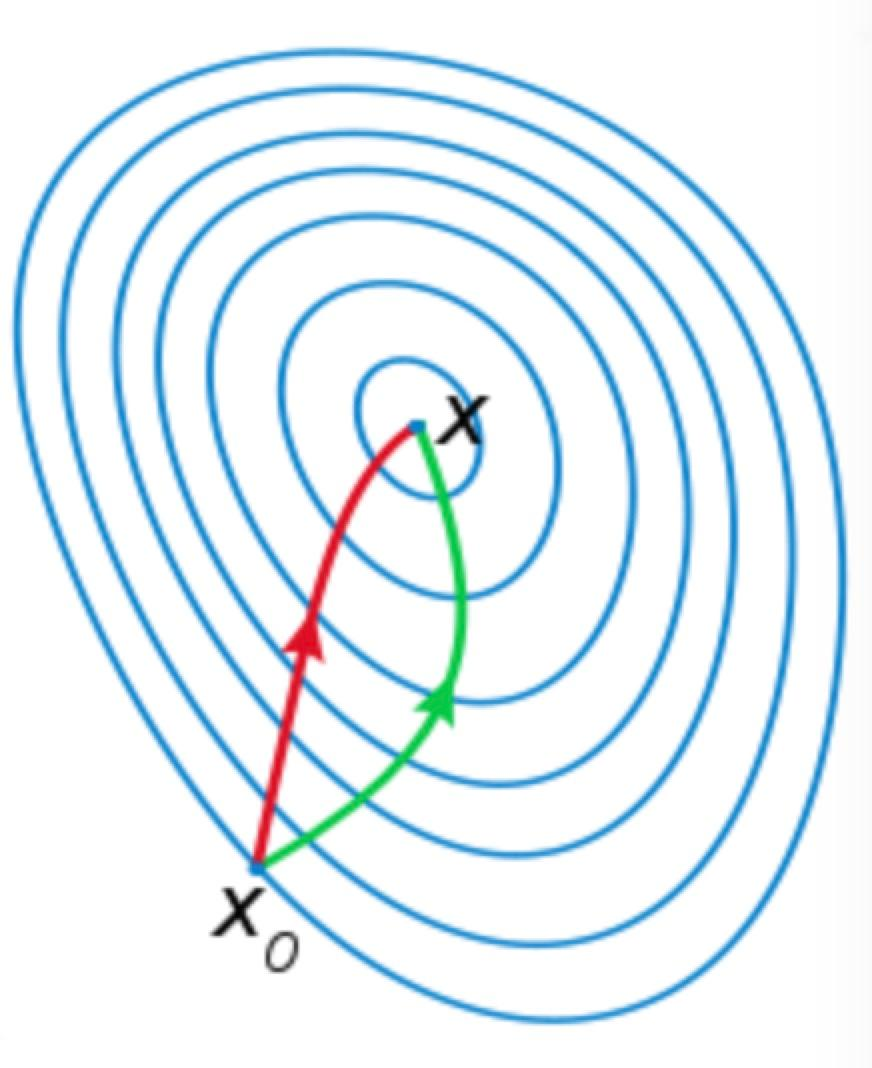
\includegraphics[height=5cm]{yijieerjie}
	\caption{红色:牛顿法 绿色:最速下降}
\end{figure}
因此可以选用另外两种更实用的方法。
\subsubsection{高斯牛顿法}
高斯牛顿法是最优化算法中比较简单的一类。我们假设目标函数$f(x)$在x处泰勒展开:
\begin{equation}
f(\boldsymbol{x}+\Delta \boldsymbol{x}) \approx f(\boldsymbol{x})+\boldsymbol{J}(\boldsymbol{x}) \Delta \boldsymbol{x}
\end{equation}
这样就在形式上跟式\ref{equ:ba}统一了,计算结果都是一个向量。我们现在计算其二范数:
\begin{equation}
e(\Delta x)=\arg \min _{\Delta x} \frac{1}{2}\|f(x)+J(x) \Delta x\|^{2}
\end{equation}
我们需要对$\Delta x$进行求导,在求导之前我们先将其展开:
\begin{equation}
\begin{aligned}
\frac{1}{2}\|f(x)+J(x) \Delta x\|^{2}=&\frac{1}{2}(f(\boldsymbol{x})+\boldsymbol{J}(\boldsymbol{x}) \Delta \boldsymbol{x})^{\mathrm{T}}(f(\boldsymbol{x})+\boldsymbol{J}(\boldsymbol{x}) \Delta \boldsymbol{x})\\
=&\frac{1}{2}\left(\|f(\boldsymbol{x})\|_{2}^{2}+2 f(\boldsymbol{x})^{\mathrm{T}} \boldsymbol{J}(\boldsymbol{x}) \Delta \boldsymbol{x}+\Delta \boldsymbol{x}^{\mathrm{T}} \boldsymbol{J}(\boldsymbol{x})^{\mathrm{T}} \boldsymbol{J}(\boldsymbol{x}) \Delta \boldsymbol{x}\right)
\end{aligned}
\end{equation}
然后再求导,令导函数为0:
\begin{equation}
2 \boldsymbol{J}(x)^{\mathrm{T}} f(\boldsymbol{x})+2 \boldsymbol{J}(\boldsymbol{x})^{\mathrm{T}} \boldsymbol{J}(\boldsymbol{x}) \Delta \boldsymbol{x}=\mathbf{0}
\end{equation}
化简后得:
\begin{equation}
J(x)^{\mathrm{T}} J(x) \Delta x=-J(x)^{\mathrm{T}} f(x)
\end{equation}
由于此方程求解的结果是增量$\Delta x$,因此我们称该方程为增量方程。定义左边系数为$\boldsymbol{H}$,定义右边系数矩阵为$\boldsymbol{g}$,那么就变成:
\begin{equation}
\boldsymbol{H} \Delta x=\boldsymbol{g}
\end{equation}
我们可以把$J^{\mathrm{T}} \mathrm{J}$理解为对$\boldsymbol{H}$的近似,从而省略了计算海塞矩阵的过程。因此,我们利用高斯牛顿法迭代的流程就是:
\begin{enumerate}[(a)]
	\item 给定初值$\boldsymbol{x}_0$
	\item 对于第k次迭代,求出当前的雅克比矩阵$J(x_k)$和误差$f(x_k)$
	\item 求解增量方程$\boldsymbol{H} \Delta x=\boldsymbol{g}$
	\item 若$\Delta x$足够小则停止,否则令$\boldsymbol{x}_{k+1}=\boldsymbol{x}+\Delta \boldsymbol{x}_k$,重复第2步。
\end{enumerate}\par
对于雅克比矩阵$\boldsymbol{J}(x_k)$和函数$f(x_k)$的求解是十分简单的,只需要带入x值就可以了。而求解$\boldsymbol{H}$是十分困难的。人们曾经一度认为由于求解H的复杂性,这种优化方法不能应用于SLAM系统,但是后来人们认识到了H的稀疏性,才使得求解大规模的增量方程成为可能。这种方法有一个问题,当通过增量方程求解出来的$\Delta x$过大的时候,就不满足泰勒展开的要求,这样一来就不能保证迭代收敛,甚至误差变的更大也有可能。列文伯格-马夸尔特(LM)方法一定程度上修正了这些问题,在SLAM里也广为应用。
\subsubsection{列文伯格-马夸尔特(LM)法}
上一节提到,高斯牛顿法当$\Delta x$过大的时候,可能会出现一些问题,甚至按照这个梯度走下去误差函数反而会增大。由此我们很自然的想到,设置一个信赖区域,当$\Delta x$小于某个值的时候,就认为高斯牛顿法是可靠的,反之则不可靠。我们考虑这样定义信赖区域:
\begin{equation}
\rho=\frac{f(\boldsymbol{x}+\Delta \boldsymbol{x})-f(\boldsymbol{x})}{\boldsymbol{J}(\boldsymbol{x}) \Delta \boldsymbol{x}}
\end{equation}
也就是当实际增量和求导计算的增量比较接近的时候,认为泰勒近似的比较好,反之则调整范围,也就是:
\begin{equation}
\min _{\Delta \boldsymbol{x}_{k}} \frac{1}{2}\left\|f\left(\boldsymbol{x}_{k}\right)+\boldsymbol{J}\left(\boldsymbol{x}_{k}\right) \Delta \boldsymbol{x}_{k}\right\|^{2}, \quad \text { s.t. }\left\|D \Delta x_{k}\right\|^{2} < \mu
\end{equation}
我们设置了信赖区域$\mu$,也就是把问题变成了一个有约束的优化问题。我们可以引入拉格朗日乘子将其重新变成无约束问题:
\begin{equation}
\min _{\Delta x_{k}} \frac{1}{2}\left\|f\left(x_{k}\right)+J\left(x_{k}\right) \Delta x_{k}\right\|^{2}+\frac{\lambda}{2}\|D \Delta x\|^{2}
\end{equation}
这里的$\lambda$是拉格朗日算子,$\boldsymbol{D}$可以看做单位阵$\boldsymbol{I}$,上式对$\Delta x$求导,相当于求解:
\begin{equation}
(H+\lambda I) \Delta x=g
\end{equation}
当参数$\lambda$较小时,$\boldsymbol{H}$占主要地位,此方法更接近高斯牛顿法,当参数$\lambda$较大时,此方法更接近最速下降法。总之,LM方法能够提供更稳定,更准确的$\Delta x$














% !TeX root = ../main.tex
\chapter{后端优化}


% !TeX root = ../main.tex

\chapter{简介}

\section{一级节标题}

\subsection{二级节标题}

\subsubsection{三级节标题}

\paragraph{四级节标题}

\subparagraph{五级节标题}

Lorem ipsum dolor sit amet, consectetur adipiscing elit, sed do eiusmod tempor
incididunt ut labore et dolore magna aliqua.
Ut enim ad minim veniam, quis nostrud exercitation ullamco laboris nisi ut
aliquip ex ea commodo consequat.
Duis aute irure dolor in reprehenderit in voluptate velit esse cillum dolore eu
fugiat nulla pariatur.
Excepteur sint occaecat cupidatat non proident, sunt in culpa qui officia
deserunt mollit anim id est laborum.



\section{脚注}

Lorem ipsum dolor sit amet, consectetur adipiscing elit, sed do eiusmod tempor
incididunt ut labore et dolore magna aliqua.
\footnote{Ut enim ad minim veniam, quis nostrud exercitation ullamco laboris
  nisi ut aliquip ex ea commodo consequat.
  Duis aute irure dolor in reprehenderit in voluptate velit esse cillum dolore
  eu fugiat nulla pariatur.}

% !TeX root = ../main.tex

\chapter{浮动体}

\section{三线表}

三线表是《撰写手册》推荐使用的格式,如表~\ref{tab:exampletable}。
\begin{table}[htb]
  \centering\small
  \caption{表号和表题在表的正上方}
  \label{tab:exampletable}
  \begin{tabular}{cl}
    \toprule
    类型   & 描述                                       \\
    \midrule
    挂线表 & 挂线表也称系统表、组织表,用于表现系统结构 \\
    无线表 & 无线表一般用于设备配置单、技术参数列表等   \\
    卡线表 & 卡线表有完全表,不完全表和三线表三种       \\
    \bottomrule
  \end{tabular}
  \note{注:表注分两种,第一种是对全表的注释,用不加阿拉伯数字排在表的下边,
    前面加“注:”;第二种是和表内的某处文字或数字相呼应的注,
    在表里面用带圈的阿拉伯数字在右上角标出,然后在表下面用同样的圈码注出来}
\end{table}

编制表格应简单明了,表达一致,明晰易懂,表文呼应、内容一致。
排版时表格字号略小,或变换字体,尽量不分页,尽量不跨节。
表格太大需要转页是,需要在续表上方注明“续表”,表头页应重复排出。



\section{插图}

有的同学可能听说“\LaTeX{} 只能使用 eps 格式的图片”,甚至把 jpg 格式转为 eps。
事实上,这种做法已经过时。
而且每次编译时都要要调用外部工具解析 eps,导致降低编译速度。
所以我们推荐矢量图直接使用 pdf 格式,位图使用 jpeg 或 png 格式。
\begin{figure}[htb]
  \centering
  \includegraphics[width=0.3\textwidth]{ustc_logo_fig.pdf}
  \caption{图号、图题置于图的下方}
  \label{fig:logo}
  \note{注:图注的内容不宜放到图题中。}
\end{figure}

关于图片的并排,推荐使用较新的 \pkg{subcaption} 宏包,
不建议使用 \pkg{subfigure} 或 \pkg{subfig} 等宏包。



\section{算法环境}

模板中使用 \pkg{algorithm2e} 宏包实现算法环境。关于该宏包的具体用法,
请阅读宏包的官方文档。

\begin{algorithm}[htb]
  \small
  \SetAlgoLined
  \KwData{this text}
  \KwResult{how to write algorithm with \LaTeX2e }

  initialization\;
  \While{not at end of this document}{
    read current\;
    \eIf{understand}{
      go to next section\;
      current section becomes this one\;
    }{
      go back to the beginning of current section\;
    }
  }
  \caption{算法示例1}
  \label{algo:algorithm1}
\end{algorithm}

注意,我们可以在论文中插入算法,但是插入大段的代码是愚蠢的。
然而这并不妨碍有的同学选择这么做,对于这些同学,建议用 \pkg{listings} 宏包。

% !TeX root = ../main.tex

\chapter{数学}

\section{数字和单位}

宏包 \pkg{siunitx} 提供了更好的数字和单位支持:
\begin{itemize}
  \item \num{12345.67890}
  \item \num{1+-2i}
  \item \num{.3e45}
  \item \num{1.654 x 2.34 x 3.430}
  \item \si{kg.m.s^{-1}}
  \item \si{\micro\meter} $\si{\micro\meter}$
  \item \si{\ohm} $\si{\ohm}$
  \item \numlist{10;20}
  \item \numlist{10;20;30}
  \item \SIlist{0.13;0.67;0.80}{\milli\metre}
  \item \numrange{10}{20}
  \item \SIrange{10}{20}{\degreeCelsius}
\end{itemize}



\section{数学符号和公式}

\LaTeX{} 默认按照美国的习惯排版数学公式和符号,
但是《撰写手册》要求数学符号依据《GB 3102.11--1993》执行,
与 \LaTeX{} 的习惯有所差异。
本模板基于 \pkg{unicode-math} 配置数学符号,以遵循国标的规定。

注意,\pkg{unicode-math} 宏包与 \pkg{amsfonts}, \pkg{amssymb}, \pkg{bm},
\pkg{mathrsfs}, \pkg{upgreek} 等宏包\emph{不}兼容。
本模板作了处理,用户可以直接使用这些宏包的命令,如 \cs{bm}, \cs{mathscr},
\cs{upGamma}。

本模板中数学符号的用法与 \LaTeX{} 传统有些区别:
\begin{itemize}
  \item 数学常数和特殊函数使用正体,
    如圆周率 $\symup{\pi}$、$\symup{\Gamma}$ 函数。
    应使用 \pkg{unicode-math} 宏包提供的 \cs{symup} 命令转为正体,
    如 \verb|\symup{\pi}|。
  \item 向量和矩阵粗斜体,应使用 \cs{symbf} 命令,
    如 \verb|\symbf{u}|、\verb|\symbf{A}|。
  \item 有限增量符号 $\increment$ (U+2206)应使用 \cs{increment} 命令。
  \item 微分符号 $\dif$ 使用正体,本模板提供了 \cs{dif} 命令。
\end{itemize}

除此之外,模板还提供了一些命令方便使用:
\begin{itemize}
  \item 常数 $\upe$:\verb|\upe|
  \item 负数单位 $\upi$:\verb|\upi|
  \item 圆周率 $\uppi$:\verb|\uppi|
  \item $\argmax$:\verb|\argmax|
  \item $\argmin$:\verb|\argmin|
\end{itemize}

关于数学符号更多的用法,参见 \pkg{unicode-math} 宏包的使用说明和符号列表
\pkg{unimath-symbols}。

在编辑数学公式时,最好避免直接使用字体命令,
而应该定义一些语义命令取代字体命令,
这样输入更简单,也让 \LaTeX{} 代码更有可读性,
而且还方便根据需要统一修改改格式,比如:
\begin{itemize}
  \item 向量 $\vec{x}$:\verb|\renewcommand\vec{\symbf}|
  \item 矩阵 $\mat{A}$:\verb|\newcommand\mat{\symbf}|
  \item 张量 $\ts{T}$: \verb|\newcommand\ts{\symbfsf}|
\end{itemize}

更多的例子:
\begin{equation}
  \upe^{\upi\uppi} + 1 = 0
\end{equation}
\begin{equation}
  \frac{\dif^2 u}{\dif t^2} = \int f(x) \dif x
\end{equation}
\begin{equation}
  \argmin_x f(x)
\end{equation}
\begin{equation}
  \mat{A} \vec{x} = \lambda \vec{x}
\end{equation}



\section{定理和证明}

示例文件中使用 \pkg{amsthm} 宏包配置了定理、引理和证明等环境。
用户也可以使用  \pkg{ntheorem} 宏包。

\begin{definition}
  If the integral of function $f$ is measurable and non-negative, we define
  its (extended) \textbf{Lebesgue integral} by
  \begin{equation}
    \int f = \sup_g \int g,
  \end{equation}
  where the supremum is taken over all measurable functions $g$ such that
  $0 \le g \le f$, and where $g$ is bounded and supported on a set of
  finite measure.
\end{definition}

\begin{assumption}
The communication graph is strongly connected.
\end{assumption}

\begin{example}
  Simple examples of functions on $\real^d$ that are integrable
  (or non-integrable) are given by
  \begin{equation}
    f_a(x) =
    \begin{cases}
      |x|^{-a} & \text{if } |x| \le 1, \\
      0        & \text{if } x > 1.
    \end{cases}
  \end{equation}
  \begin{equation}
    F_a(x) = \frac{1}{1 + |x|^a}, \qquad \text{all } x \in \real^d.
  \end{equation}
  Then $f_a$ is integrable exactly when $a < d$, while $F_a$ is integrable
  exactly when $a > d$.
\end{example}

\begin{lemma}[Fatou]
  Suppose $\{f_n\}$ is a sequence of measurable functions with $f_n \geq 0$.
  If $\lim_{n \to \infty} f_n(x) = f(x)$ for a.e. $x$, then
  \begin{equation}
    \int f \le \liminf_{n \to \infty} \int f_n.
  \end{equation}
\end{lemma}

\begin{remark}
  We do not exclude the cases $\int f = \infty$,
  or $\liminf_{n \to \infty} f_n = \infty$.
\end{remark}

\begin{corollary}
  Suppose $f$ is a non-negative measurable function, and $\{f_n\}$ a sequence
  of non-negative measurable functions with
  $f_n(x) \le f(x)$ and $f_n(x) \to f(x)$ for almost every $x$. Then
  \begin{equation}
    \lim_{n \to \infty} \int f_n = \int f.
  \end{equation}
\end{corollary}

\begin{proposition}
  Suppose $f$ is integrable on $\real^d$. Then for every $\epsilon > 0$:
  \begin{enumerate}
    \renewcommand{\theenumi}{\roman{enumi}}
    \item There exists a set of finite measure $B$ (a ball, for example) such
      that
      \begin{equation}
        \int_{B^c} |f| < \epsilon.
      \end{equation}
    \item There is a $\delta > 0$ such that
      \begin{equation}
        \int_E |f| < \epsilon \qquad \text{whenever } m(E) < \delta.
      \end{equation}
  \end{enumerate}
\end{proposition}

\begin{theorem}
  Suppose $\{f_n\}$ is a sequence of measurable functions such that
  $f_n(x) \to f(x)$ a.e. $x$, as $n$ tends to infinity.
  If $|f_n(x)| \le g(x)$, where $g$ is integrable, then
  \begin{equation}
    \int |f_n - f| \to 0 \qquad \text{as } n \to \infty,
  \end{equation}
  and consequently
  \begin{equation}
    \int f_n \to \int f \qquad \text{as } n \to \infty.
  \end{equation}
\end{theorem}

\begin{proof}
  Trivial.
\end{proof}

\newtheorem*{axiomofchoice}{Axiom of choice}
\begin{axiomofchoice}
  Suppose $E$ is a set and ${E_\alpha}$ is a collection of
  non-empty subsets of $E$. Then there is a function $\alpha
  \mapsto x_\alpha$ (a ``choice function'') such that
  \begin{equation}
    x_\alpha \in E_\alpha,\qquad \text{for all }\alpha.
  \end{equation}
\end{axiomofchoice}

\newtheorem{observation}{Observation}
\begin{observation}
  Suppose a partially ordered set $P$ has the property
  that every chain has an upper bound in $P$. Then the
  set $P$ contains at least one maximal element.
\end{observation}
\begin{proof}[A concise proof]
  Obvious.
\end{proof}

% !TeX root = ../main.tex

\chapter{引用文献的标注}

模板使用 \pkg{natbib} 宏包来设置参考文献引用的格式,
更多引用方法可以参考该宏包的使用说明。



\section{顺序编码制}

\subsection{角标数字标注法}

\citestyle{super}
\noindent
\begin{tabular}{l@{\quad$\Rightarrow$\quad}l}
  \verb|\cite{knuth86a}|         & \cite{knuth86a}         \\
  \verb|\citet{knuth86a}|        & \citet{knuth86a}        \\
  \verb|\cite[42]{knuth86a}|     & \cite[42]{knuth86a}     \\
  \verb|\cite{knuth86a,tlc2}|    & \cite{knuth86a,tlc2}    \\
  \verb|\cite{knuth86a,knuth84}| & \cite{knuth86a,knuth84} \\
\end{tabular}


\subsection{数字标注法}

\citestyle{numbers}
\noindent
\begin{tabular}{l@{\quad$\Rightarrow$\quad}l}
  \verb|\cite{knuth86a}|         & \cite{knuth86a}         \\
  \verb|\citet{knuth86a}|        & \citet{knuth86a}        \\
  \verb|\cite[42]{knuth86a}|     & \cite[42]{knuth86a}     \\
  \verb|\cite{knuth86a,tlc2}|    & \cite{knuth86a,tlc2}    \\
  \verb|\cite{knuth86a,knuth84}| & \cite{knuth86a,knuth84} \\
\end{tabular}



\section{著者-出版年制标注法}

\citestyle{authoryear}
\noindent
\begin{tabular}{l@{\quad$\Rightarrow$\quad}l}
  \verb|\cite{knuth86a}|         & \cite{knuth86a}         \\
  \verb|\citep{knuth86a}|        & \citep{knuth86a}        \\
  \verb|\cite[42]{knuth86a}|     & \cite[42]{knuth86a}     \\
  \verb|\cite{knuth86a,tlc2}|    & \cite{knuth86a,tlc2}    \\
  \verb|\cite{knuth86a,knuth84}| & \cite{knuth86a,knuth84} \\
\end{tabular}

\vskip 2ex \citestyle{super}
注意,参考文献列表中的每条文献在正文中都要被引用
\cite{slg,lyc,ljs,cgw,cjb,kqy,yhs,yx,dwx,jxz,wjk,syw,wf,xd,twh,huston}。

\bibliography{bib/ustc}

\appendix
% !TeX root = ../main.tex

\chapter{补充材料}


补充内容。


\backmatter
% !TeX root = ../main.tex

\begin{acknowledgements}

在研究学习期间,我有幸得到了三位老师的教导,
他们是:我的导师,中国科大XXX研究员,中科院X昆明动物所马老师以及美国犹他大学的XXX老师。
三位深厚的学术功底,严谨的工作态度和敏锐的科学洞察力使我受益良多。
衷心感谢他们多年来给予我的悉心教导和热情帮助。

感谢XXX老师在实验方面的指导以及教授的帮助。
科大的XXX同学和XXX同学参与了部分试验工作,在此深表谢意。

\end{acknowledgements}

% !TeX root = ../main.tex

\begin{publications}

\section*{已发表论文}

\begin{enumerate}
\item A A A A A A A A A
\item A A A A A A A A A
\item A A A A A A A A A
\end{enumerate}

\section*{待发表论文}

\begin{enumerate}
\item A A A A A A A A A
\item A A A A A A A A A
\item A A A A A A A A A
\end{enumerate}

\section*{研究报告}
\begin{enumerate}
\item A A A A A A A A A
\item A A A A A A A A A
\item A A A A A A A A A
\end{enumerate}

\end{publications}


\end{document}
